%%% Local Variables:
%%% mode: latex
%%% TeX-master: t
%%% End:

\documentclass{article}

%%% Package imports
\usepackage[utf8]{inputenc}
\usepackage[ruled]{algorithm2e}
\usepackage{hyperref}
\usepackage{amsmath}
\usepackage{zed-csp}
\usepackage{breqn}
\usepackage{xcolor}
\usepackage{listings}
\usepackage{pgfplots}
\usepackage{pgfplotstable}
\pgfplotsset{compat=newest}
\usepgfplotslibrary{dateplot}
\usepgfplotslibrary{polar}
\usetikzlibrary{pgfplots.dateplot}
\usetikzlibrary{pgfplots.patchplots}
\usetikzlibrary{patterns}

\usepackage{graphicx}
\usepackage{floatrow}

\usepackage{calc}
\makeatletter\@mparswitchfalse\makeatother
\DeclareMarginSet{hangleft}{\setfloatmargins
{\hskip-\marginparwidth\hskip-\marginparsep}{\hfil}}
\floatsetup[widefigure]{margins=hangleft}
%%% ^ Figure formatting within Appendex A

\lstset{literate = {-}{-}1} % get dashs to show up

%%% https://tex.stackexchange.com/questions/195486/how-can-i-highlight-json-string-values-but-not-attributes/195540#195540
%%% ^ JSON style for lstset
\newcommand\JSONnumbervaluestyle{\color{blue}}
\newcommand\JSONstringvaluestyle{\color{red}}
\newif\ifcolonfoundonthisline
\makeatletter

\lstdefinestyle{json}
{
  showstringspaces    = false,
  keywords            = {false,true},
  alsoletter          = 0123456789.,
  morestring          = [s]{"}{"},
  stringstyle         = \ifcolonfoundonthisline\JSONstringvaluestyle\fi,
  MoreSelectCharTable =%
  \lst@DefSaveDef{`:}\colon@json{\processColon@json},
  basicstyle          = \ttfamily,
  keywordstyle        = \ttfamily\bfseries,
}

\newcommand\processColon@json{%
  \colon@json%
  \ifnum\lst@mode=\lst@Pmode%
  \global\colonfoundonthislinetrue%
  \fi
}

\lst@AddToHook{Output}{%
  \ifcolonfoundonthisline%
  \ifnum\lst@mode=\lst@Pmode%
  \def\lst@thestyle{\JSONnumbervaluestyle}%
  \fi
  \fi
  % override by keyword style if a keyword is detected!
  \lsthk@DetectKeywords%
}

% reset the switch at the end of line
\lst@AddToHook{EOL}%
{\global\colonfoundonthislinefalse}

\makeatother
\pgfplotsset{compat=1.15}

\title{Data Analytics and Visualization Efficiency Framework for xAPI and the Total Learning Architecture: DAVE Learning Analytics Algorithms}
\author{Yet Analytics}

\begin{document}

\begin{titlepage}
  \maketitle
\end{titlepage}

\section*{Introduction}
This report introduces the initial learning analytics algorithms,
\textbf{timeline of learner success},\textbf{which assessment
  questions are the most difficult} and \textbf{rate of completions}
of the DAVE Framework. In doing so, it establishes a set of style
guidelines for the reporting of algorithms and associated
visualization templates necessary to work with the DAVE
Framework. This document will be updated to include the learning
analytics questions defined within the
\href{https://adloffice365.sharepoint.com/sites/TLA_Extranet/Shared\%20Documents/2018\%20TLA\%20Data\%20Requirements\%20Aligned\%20to\%20Event.docx?d=w1cf1d6fe161b4606a11c130baae5f5e1}{2018
  TLA Data Requirements} document in addition to other learning
analytics algorithms which have yet to be defined. Updates may also
address refinement of these algorithms and this document should be
understood to be an example of algorithm presentation and not the
final state of any defined algorithm.

$\\\\$
The structure of this documents is as follows:
\begin{enumerate}
\item A formal specification for xAPI written in Z
  and referenced within the formal specifications of learning
  analytics algorithms
\item An algorithm definition which will consist of:
  \begin{enumerate}
  \item an introduction for the algorithm
  \item the structure of the ideal input data
  \item how to retrieve input data from an LRS
  \item the statement parameters which the algorithm will utilize
  \item notices regarding data collected during the 2018 pilot test of
    the TLA
  \item a summary of the algorithm
  \item the formal specification of the algorithm
  \item pseudocode representation of the algorithm
  \item JSONSchema for the output of the algorithm
  \item a description of the associated visualization
  \item a prototype of the visualization
  \item a collection of suggestions describing how the algorithm could be
    adapted to improve the quality of the visualization prototype
  \end{enumerate}
\end{enumerate}
$\\\\\\\\\\\\$ %%% only introduction on the first page
\section{xAPI Formal Specification}
The current formal specification only defines xAPI statements
abstractly within the context of Z. A concrete definition for xAPI
statements is outside the scope of this document.

\subsection{Basic Types}
$IFI$ ::=$ mbox \,|\, mbox\_sha1sum \,|\, openid \,|\, account$
\begin{itemize}
\item Type unique to Agents and Groups, The concrete definition of the listed values
  is outside the scope of this specification
\end{itemize}
$OBJECTTYPE$ ::=$ Agent \,|\, Group \,|\, SubStatement \,|\,
StatementRef \,|\, Activity$
\begin{itemize}
\item A type which can be present in all activities as defined by
  the xAPI specification
\end{itemize}
$INTERACTIONTYPE$ ::= $true-false \,|\, choice \,|\, fill-in \,|\,
long-fill-in \,|\, matching \,| \\ performance \,|\, sequencing \,|\,
likert \,|\, numeric \,|\, other$
\begin{itemize}
\item A type which represents the possible interactionTypes as
  defined within the xAPI specification
\end{itemize}
$INTERACTIONCOMPONENT$ ::= $choices \,|\, scale \,|\, source \,|\,
target \,|\, steps$
\begin{itemize}
\item A type which represents the possible interaction components as
  defined within the xAPI specification
\item the concrete definition of the listed values is outside the
  scope of this specification
\end{itemize}
$CONTEXTTYPES$ ::= $parent \,|\, grouping \,|\, category \,|\, other$
\begin{itemize}
\item A type which represents the possible context types as
  defined within the xAPI specification
\end{itemize}
$[STATEMENT]$
\begin{itemize}
\item Basic type for an xAPI data point
\end{itemize}
$[AGENT, GROUP]$
\begin{itemize}
\item Basic types for Agents and collections of Agents
\end{itemize}

\subsection{Id Schema}
\begin{schema}{Id}
  id : \finset_1 \#1
\end{schema}
\begin{itemize}
\item the schema $Id$ introduces the component $id$ which is a
  non-empty, finite set of 1 value
\end{itemize}

\subsection{Schemas for Agents, Groups and Actors}

\begin{schema}{Agent}
  agent : AGENT \\
  objectType : OBJECTTYPE \\
  name : \finset_1 \#1 \\
  ifi : IFI
  \where
  objectType = Agent \\
  agent = \{ifi\} \cup \power \{name, objectType\}
\end{schema}
\begin{itemize}
\item The schema $Agent$ introduces the component $agent$ which is a set
  consisting of an $ifi$ and optionally an $objectType$ and/or $name$
\end{itemize}

\begin{schema}{Member}
  Agent \\
  member : \finset_1
  \where
  member = \{a : AGENT \,|\, \forall a_{n}: a_{i}..a_{j} @ i \leq n
  \leq j @ a = agent\}
\end{schema}
\begin{itemize}
\item The schema $Member$ introduces the component $member$ which is a set of
  objects $a$, where for every $a$ within $a_{0}..a_{n}$, $a$ is an $agent$
\end{itemize}

\begin{schema}{Group}
  Member \\
  group : GROUP \\
  objectType : OBJECTTYPE \\
  ifi : IFI\\
  name : \finset_1 \#1
  \where
  objectType = Group \\
  group = \{objectType, name, member\} \lor \{objectType, member\}
  \lor \\ \t2 \{objectType, ifi\} \cup \power \{name, member\}
\end{schema}
\begin{itemize}
\item The schema $Group$ introduces the component $group$ which is of
  type $GROUP$ and is a set of either $objectType$ and $member$ with optionaly $name$ or
  $objectType$ and $ifi$ with optionally $name$ and/or $member$
\end{itemize}

\begin{schema}{Actor}
  Agent \\
  Group \\
  actor : AGENT \lor GROUP
  \where
  actor = agent \lor group
\end{schema}
\begin{itemize}
\item The schema $Actor$ introduces the component $actor$ which
  is either an $agent$ or $group$
\end{itemize}

\subsection{Verb Schema}
\begin{schema}{Verb}
  Id \\
  display, verb : \finset_1
  \where
  verb = \{id, display\} \lor \{id\}
\end{schema}
\begin{itemize}
\item The schema $Verb$ introduces the component $verb$ which
  is a set that consists of either $id$ and the non-empty, finite set
  $display$ or just $id$
\end{itemize}

\subsection{Object Schema}

\begin{schema}{Extensions}
  extensions, extensionVal : \finset_1 \\
  extensionId : \finset_1 \#1 \\
  \where
  extensions = \{e : (extensionId, extensionVal)\ \,|\,
  \forall e_{n} : e_{i}..e_{j} @ i \leq n \leq j @ \\
  \t3 \, (extensionId_{i}, extensionVal_{i})
  \lor (extensionId_{i}, extensionVal_{j}) \land \\
  \t3 \, (extensionId_{j}, extensionVal_{i})
  \lor (extensionId_{j}, extensionVal_{j})
  \land \\ \t3 \, extensionId_{i} \not = extensionId_{j}\}
\end{schema}
\begin{itemize}
\item The schema $Extensions$ introduces the component $extensions$ which
  is a non-empty, finite set that consists of ordered pairs of
  $extensionId$ and $extensionVal$. Different $extensionId$s can
  have the same $extensionVal$ but there can not be two identical
  $extensionId$ values
\item $extensionId$ is a non-empty, finite set with one value
\item $extensionVal$ is a non-empty, finite set
\end{itemize}

\begin{schema}{InteractionActivity}
  interactionType : INTERACTIONTYPE \\
  correctResponsePattern : \seq_1 \\
  interactionComponent: INTERACTIONCOMPONENT \\
  \where
  interactionActivity = \{interactionType, correctReponsePattern,
  interactionComponent\} \lor \\ \t5 \{interactionType, correctResponsePattern\}
\end{schema}
\begin{itemize}
\item The schema $InteractionActivity$ introduces the component
  $interactionActivity$ which is a set of either $interactionType$
  and $correctResponsePattern$ or $interactionType$ and
  $correctResponsePattern$ and $interactionComponent$
\end{itemize}

\begin{schema}{Definition}
  InteractionActivity \\
  Extensions \\
  definition, name, description : \finset_1 \\
  type, moreInfo : \finset_1 \#1
  \where
  definition = \power_1 \{name, description, type, moreInfo,
  extensions, interactionActivity\} \\
\end{schema}
\begin{itemize}
\item The schema $Definition$ introduces the component
  $definition$ which is the non-empty, finite power set of $name$, $description$,
  $type$, $moreInfo$ and $extensions$
\end{itemize}

\begin{schema}{Object}
  Id \\
  Definition \\
  Agent \\
  Group \\
  Statement \\
  objectTypeA, objectTypeS, objectTypeSub, objectType  : OBJECTTYPE \\
  substatement : STATEMENT \\
  object : \finset_1 \\
  \where
  substatement = statement \\
  objectTypeA = Activity \\
  objectTypeS = StatementRef \\
  objectTypeSub = SubStatement \\
  objectType = objectTypeA \lor objectTypeS \\
  object = \{id\} \lor \{id, objectType\} \lor \{id, objectTypeA,
  definition\} \\ \t2 \lor \{id, definition\} \lor \{agent\} \lor
  \{group\} \lor \{objectTypeSub, substatement\} \\
  \t2 \lor \{id, objectTypeA\}
\end{schema}
\begin{itemize}
\item The schema $Object$ introduces the component $object$ which
  is a non-empty, finite set of either $id$, $id$ and $objectType$,
  $id$ and $objectTypeA$, $id$ and $objectTypeA$ and $definition$,
  $agent$, $group$, or $substatement$
\item The schema $Statement$ and the corresponding component
  $statement$ will be defined later on in this specification
\end{itemize}
$\\\\\\\\\\\\$ %%% Header with content
\subsection{Result Schema}

\begin{schema}{Score}
  score : \finset_1 \\
  scaled, min, max, raw : \num \\
  \where
  scaled = \{ n : \num \,|\, -1.0 \leq n \leq 1.0 \} \\
  min = n < max \\
  max = n > min \\
  raw = \{ n : \num \,|\, min \leq n \leq max \} \\
  score = \power_1 \{scaled, raw, min, max\}
\end{schema}
\begin{itemize}
\item The schema $Score$ introduces the component $score$ which is
  the non-empty powerset of $min$, $max$, $raw$ and $scaled$
\end{itemize}

\begin{schema}{Result}
  Score \\
  Extensions \\
  success, completion, response, duration : \finset_1 \#1 \\
  result : \finset_1
  \where
  success = \{true\} \lor \{false\} \\
  completion = \{true\} \lor \{false\} \\
  result = \power_1 \{score, success, completion, response,
  duration, extensions\}
\end{schema}
\begin{itemize}
\item The schema $Result$ introduces the component $result$ which is
  the non-empty power set of $score$, $success$, $completion$,
  $response$, $duration$ and $extensions$
\end{itemize}

\subsection{Context Schema}

\begin{schema}{Instructor}
  Agent \\
  Group \\
  instructor : AGENT \lor GROUP
  \where
  instructor = agent \lor group
\end{schema}
\begin{itemize}
\item The schema $Instructor$ introduces the component $instructor$
  which can be ether an $agent$ or a $group$
\end{itemize}

\begin{schema}{Team}
  Group \\
  team : GROUP
  \where
  team = group
\end{schema}
\begin{itemize}
\item The schema $Team$ introduces the component $team$ which is a $group$
\end{itemize}

\begin{schema}{Context}
  Instructor \\
  Team \\
  Object \\
  Extensions \\
  registration, revision, platform, language : \finset_1 \#1 \\
  parentT, groupingT, categoryT, otherT : CONTEXTTYPES \\
  contextActivities, statement : \finset_1
  \where
  statement = object \hide (id, objectType, agent, group,
  definition) \\
  parentT = parent \\
  groupingT = grouping \\
  categoryT = category \\
  otherT = other \\
  contextActivity = \{ca : object \hide (agent, group, objectType,
  objectTypeSub, substatement)\} \\
  contextActivityParent = (parentT, contextActivity) \\
  contextActivityCategory = (categoryT, contextActivity) \\
  contextActivityGrouping = (groupingT, contextActivity) \\
  contextActivityOther = (otherT, contextActivity) \\
  contextActivities = \power_1 \{contextActivityParent,
  contextActivityCategory, \\ \t5 \:\: contextActivityGrouping,
  contextActivityOther\} \\
  context = \power_1 \{registration, instructor, team,
  contextActivities, revision, \\ \t3 platform, language, statement, extensions\}
\end{schema}
\begin{itemize}
\item The schema $Context$ introduces the component $context$
  which is the non-empty powerset of $registration$, $instructor$,
  $team$, $contextActivities$, $revision$, $platform$, $language$,
  $statement$ and $extensions$
\item The notation $object \hide agent$ represents the component
  $object$ except for its subcomponent $agent$
\end{itemize}

\subsection{Timestamp and Stored Schema}

\begin{schema}{Timestamp}
  timestamp : \finset_1 \#1
\end{schema}

\begin{schema}{Stored}
  stored : \finset_1 \#1
\end{schema}
\begin{itemize}
\item The schema $Timestamp$ and $stored$ introduce the components
  $timestamp$ and $stored$ respectively. Each are non-empty, finite
  sets containing one value
\end{itemize}

\subsection{Attachements Schema}

\begin{schema}{Attachments}
  display, description, attachment, attachments: \finset_1 \\
  usageType, sha2, fileUrl, contexntType : \finset_1 \#1 \\
  length : \nat
  \where
  attachment = \{usageType, display, contentType, length, sha2 \}
  \cup \power \{description, fileUrl\} \\
  attachments = \{a : attachment\}
\end{schema}
\begin{itemize}
\item The schema $Attachements$ introduces the componenet
  $attachements$ which is a non-empty, finite set of the component
  $attachement$
\item The component $attachment$ is a non-empty, finite set of the
  componenets $usageType$, $display$, $contentType$, $length$,
  $sha2$ with optionally $description$ and/or $fileUrl$
\end{itemize}

\subsection{Statement and Statements Schema}

\begin{schema}{Statement}
  Id \\
  Actor \\
  Verb \\
  Object \\
  Result \\
  Context \\
  Timestamp \\
  Stored \\
  Attachements \\
  statement : STATEMENT

  \where
  statement = \{actor, verb, object, stored\} \cup \\\t3 \power \{\id,
  result, context, timestamp, attachments \} \\
\end{schema}
\begin{itemize}
\item The schema $Statement$ introduces the component $statement$
  which consists of the components $actor$, $verb$, $object$ and
  $stored$ and the optional components $id$, $result$, $context$,
  $timestamp$, and/or $attachments$
\item The schema $Statement$ allows for subcomponent of $statement$
  to refrenced via the $.$ (selection) operator
\end{itemize}

\begin{schema}{Statements}
  Statement \\
  IsoToUnix \\
  statements : \finset_1
  \where
  statements = \{s : statement \,|\, \forall s_{n}: s_{i}..s_{j} @ i
  \leq n \leq j \\\t3\: @ convert(s_{i}.timestamp) \leq convert(s_{j}.timestamp) \}
\end{schema}
\begin{itemize}
\item The schema $Statements$ introduces the component $statements$
  which is a non-empty, finite set of the component $statement$ which
  are in chronological order.
\end{itemize}

\section{Timeline Of Learner Success}
As learners engage in activities supported by a learning ecosystem, they will build
up a history of learning experiences. When the digital resources of that learning ecosystem
adhere to a framework dedicated to supporting and understanding the
learner, such as the Total Learning Architecture (TLA), it becomes
possible to retell their learning story through data and data visualization. One important aspect of
that story is the' learners history of success.

\subsection{Ideal Statements}
In order to accurately portray a learner's timeline of success, there
are a few base requirements of the data produced by a Learning Record
Provider (LRP). They are as follows:

\begin{itemize}
\item the learner must be uniquely and consistently identified across
  all statements
\item learning activities which evaluate a learner's understanding of material must report if the learner was successful or not
  \begin{itemize}
  \item the grade earned by the learner must be reported
  \item the minimum and maximum possible grade must be reported
  \end{itemize}
\item The learning activities must be uniquely and consistently identified across all statements
\item The time at which a learner completed a learning activity must be recorded
  \begin{itemize}
  \item The timestamp should contain an appropriate level of specificity.
  \item ie. Year, Month, Day, Hour, Minute, Second, Timezone
  \end{itemize}
\end{itemize}

\subsection{Input Data Retrieval}
How to query an LRS via a GET request to the Statements Resource via
curl. The following section contains the appropriate parameters with
example values as well as the curl command necessary for making the
request.\footnote{\label{moreLink} $S$ is the set of all statements
  parsed from the statements array within the HTTP response to the
  Curl request(s). It may be possible that multiple Curl requests are
  needed to retrieve all query results. If multiple requests are
  necessary, $S$ is the result of concatenating the result of each
  request into a single set}\footnote{\label{noZ} Querying an LRS will
  not be defined within the following Z specifications but the results
  of the query will be utilized}\footnote{\label{allTime} If you want
  to query across the entire history of a LRS, omit Since and Until
  from the endpoint(s) and remove the associated \& symbols.}

\begin{lstlisting}[frame=single]
Agent = "agent={"account":
                {"homePage": "https://example.homepage",
                 "name": 123456}}"

Since = "since=2018-07-20T12:08:47Z"

Until = "until=2018-07-21T12:08:47Z"

Base = "https://example.endpoint/statements?"

endpoint = Base + Agent + "&" + Since + "&" + Until

Auth = Hash generated from basic auth

S = curl -X GET -H "Authorization: Auth"
         -H "Content-Type: application/json"
         -H "X-Experience-API-Version: 1.0.3"
         Endpoint
\end{lstlisting}

\subsection{Statement Parameters to Utilize}
The statement parameter locations here are written in
\href{http://goessner.net/articles/JsonPath/}{JSONPath}. This notation
is also compatable with the xAPI Z notation due to the defined
hierarchy of components. Within the Z specifications, a variable name
will be used instead of the $\$$
\begin{itemize}
\item $\$.timestamp$
\item $\$.result.success$
\item $\$.result.score.raw$
\item $\$.result.score.min$
\item $\$.result.score.max$
\item $\$.verb.id$
\end{itemize}

\subsection{2018 Pilot TLA Statement Problems}
The initial pilot test data supports this algorithm.
This section may require updates pending future data review following iterations of the TLA testing.
\subsection{Summary}
\begin{enumerate}
\item Query an LRS via a \href{https://github.com/adlnet/xAPI-Spec/blob/master/xAPI-Communication.md#213-get-statements}{GET} request to the statements endpoint using the parameters agent, since and until
\item Filter the results to the set of statements where:
  \begin{itemize}
  \item $\$.verb.id$ is one of:
    \begin{itemize}
    \item http://adlnet.gov/expapi/verbs/passed
    \item https://w3id.org/xapi/dod-isd/verbs/answered
    \item http://adlnet.gov/expapi/verbs/completed
    \end{itemize}
  \item $\$.result.success$ is true
  \end{itemize}
\item process the filtered data
  \begin{itemize}
  \item extract $\$.timestamp$
  \item extract the score values from $\$.result.score.raw$,
    $\$.result.score.min$ and $\$.result.score.max$ and convert them
    to the scale 0..100
  \item create a pair of [$\$.timestamp$, $\#$]
  \end{itemize}
\end{enumerate}

\subsection{Formal Specification}
\subsubsection{Basic Types}

$COMPLETION$ :== \\ $\{http://adlnet.gov/expapi/verbs/passed\} \, | \\
\{https://w3id.org/xapi/dod-isd/verbs/answered\} \; | \\
\{http://adlnet.gov/expapi/verbs/completed$\} \\
\\
$SUCCESS$ :== $\{true\}$

\subsubsection{System State}

\begin{schema}{TimelineLearnerSuccess}
  Statements \\
  S_{all} : \finset_1 \\
  S_{completion},S_{success},S_{processed} : \finset \\
  \where
  S_{all} = statements \\
  S_{completion} \subseteq S_{all} \\
  S_{success} \subseteq S_{completion} \\
  S_{processed} = \{pair : (statement.timestamp, \nat)\}
\end{schema}
\begin{itemize}

\item The set $S_{all}$ is a non-empty, finite set and is the
  component $statements$
\item The sets $S_{completion}$ and $S_{success}$ are both finite sets
\item the set $S_{completion}$ is a subset of $S_{all}$ which may
  contain every value within $S_{all}$
\item the set $S_{success}$ is a subset of $S_{completion}$ which may
  contain every value within $S_{completion}$
\item the set $S_{processed}$ is a finite set of pairs where each
  contains a $statement.timestamp$ and a natural number
\end{itemize}

\subsubsection{Initial System State}
\begin{schema}{InitTimelineLearnerSuccess}
  TimelineLearnerSuccess \\
  \where
  S_{all} \not = \emptyset \\
  S_{completion} = \emptyset \\
  S_{success} = \emptyset \\
  S_{processed} = \emptyset
\end{schema}
\begin{itemize}
\item The set $S_{all}$ is a non-empty set
\item The sets $S_{completion}$,\,$S_{success}$ and $S_{processed}$ are all initially empty
\end{itemize}

\subsubsection{Filter for Completion}
\begin{schema}{Completion}
  Statement \\
  completion : STATEMENT \pfun \finset \\
  s? : STATEMENT \\
  s! : \finset \\
  \where
  s? = statement \\
  s! = completion(s?) \\
  completion(s?) = \IF s?.verb.id : COMPLETION \\\t5 \THEN s! = s?
  \\\t5 \ELSE s! = \emptyset
\end{schema}
\begin{itemize}
\item The schema $Completion$ inroduces the function $completion$
  which takes in the variable $s?$ and returns the variable $s!$
\item The variable $s?$ is the component $statement$
\item $s!$ is equal to $s?$
  if $\$.verb.id$ is of the type $COMPLETION$ otherwise $s!$ is an empty set
\end{itemize}

\begin{schema}{FilterForCompletion}
  \Delta TimelineLearnerSuccess \\
  Completion \\
  completions : \finset
  \where
  completions \subseteq S_{all} \\
  completions' = \{s : STATEMENT \,|\, completion(s) \not = \emptyset\} \\
  S_{completion}' = S_{completion} \cup completions' \\
\end{schema}
\begin{itemize}
\item the set $completions$ is a subset of $S_{all}$ which may contain
  every value within $S_{all}$
\item The set $completions'$ is the set of all statements $s$ where
  the result of $completion(s)$ is not an empty set
\item the updated set $S'_{completion}$ is the union of the previous
  state of set $S_{completion}$ and the set $completions'$
\end{itemize}

\subsubsection{Filter for Success}
\begin{schema}{Success}
  Statement \\
  success : STATEMENT \pfun \finset \\
  s? : STATEMENT \\
  s! : \finset \\
  \where
  s? = statement \\
  s! = success(s?) \\
  success(s?) = \IF s?.result.success : SUCCESS \\\t4 \THEN s! = s?
  \\\t4 \ELSE s! = \emptyset
\end{schema}
\begin{itemize}
\item the schema $Success$ introduces the function $success$ which
  takes in the variable $s?$ and returns the variable $s!$
\item the variable $s?$ is the component $statement$
\item $s!$ is equal to $s?$ if $\$.result.success$ is of the type
  $SUCCESS$ otherwise $s!$ is an empty set
\end{itemize}

\begin{schema}{FilterForSuccess}
  \Delta TimelineLearnerSuccess \\
  Success \\
  successes : \finset
  \where
  successes \subseteq S_{completion} \\
  successes' = \{s : STATEMENT \,|\, success(s) \not = \emptyset\} \\
  S_{success}' = S_{success} \cup successes'
\end{schema}
\begin{itemize}
\item the set $successes$ is a subset of $S_{completion}$ which may contain
  every value within $S_{completion}$
\item The set $successes'$ contains elements $s$ of type $STATEMENT$
  where $success(s)$ is not an empty set
\item The updated set $S_{success}'$ is the union of the previous
  state of $S_{success}$ and $successes'$
\end{itemize}

\subsubsection{Processes Results}
\begin{schema}{Scale}
  scaled! : \nat \\
  raw?, min?, max? : \num \\
  scale : \num \fun \nat
  \where
  scaled! = scale(raw?, min?, max?) \\
  scale(raw?, min?, max?) = \\\t4
  (raw? * ((0.0 - 100.0) \, div \, (min? - \, max?))) \, + \\ \t4
  (0.0 - (min? * ((0.0 - 100.0) div (min? - \, max?))))
\end{schema}
\begin{itemize}
\item The schema $Scale$ introduces the function $scale$ which takes
  3 arguments, $raw?$, $min?$ and $max?$. The function converts
  $raw?$ from the range $min?..max?$ to 0.0..100.0
\end{itemize}

\begin{schema}{ProcessStatements}
  \Delta TimelineLearnerSuccess \\
  Scale \\
  FilterStatements \\
  processed : \finset
  \where
  processed \subseteq S_{success} \\
  processed' = \{p : (\finset_1\#1 , \nat) \,|\, \\\t3
  \LET \{processed_{i}..processed_{j}\} == \{s_{i}..s_{j}\} @ \\ \t3
  i \leq n \leq j @ \forall s_{n} : s_{i}..s_{j} @
  \exists \, p_{n} : p_{i}..p_{j} @ \\\t3 first~p_{n} = s_{n}.timestamp \, \land
  \\\t3 second~p_{n} = scale(s_{n}.result.score.raw, \\\t7
  s_{n}.result.score.min, \\\t7
  s_{n}.result.score.max)\} \\
  S_{processed}' = S_{processed} \cup processed'

\end{schema}
\begin{itemize}
\item The operation $ProcessStatements$ introduces the variable
  $processed$ which is a subset of $S_{success}$ which may contain
  every value within $S_{success}$
\item $S_{success}$ is the result of the operation $FilterStatements$
\item The operation defines the variable $processsed'$ which is a
  set of objects $p$ which are ordered pairs of (1) a finite set
  containing one value and (2) a single positive number.
\item The first component of every object $p$, is the
  timestamp from the associated $statement$ within $processed$
  ie. $s.timestamp$
\item The second component of every object $p$ is the result
  of the function $scale$. The score values contained within the
  associated $statement$ $s$ are the arugments passed to $scale$. ie $scale(s.result.score.raw, s.result.score.min,
  s.result.score.max)$
\item The result of the operation $ProcessStatements$ is to updated
  the set $S_{processed}$ with the values contained within $processed'$
\end{itemize}

\subsubsection{Sequence of Operations}

$FilterStatements \defs FilterForCompletion \semi FilterForSuccess$
\begin{itemize}
\item The schema $FilterStatements$ is the sequential composition
  of operation schemas $FilterForCompletion$ and
  $FilterForSuccess$
\item $FilterForCompletion$ happens before $FilterForSuccess$
\end{itemize}
%%% this fixes indenting
$ProcessedStatements \defs FilterStatements \semi ProcessStatements$
\begin{itemize}
\item The schema $ProcessedStatements$ is the sequential composition
  of operation schemas $FilterStatements$ and
  $ProcessStatements$
\item $FilterStatements$ happens before $ProcessStatements$
\end{itemize}

\subsubsection{Return}
\begin{schema}{Return}
  \Xi TimelineLearnerSuccess \\
  ProcessedStatements \\
  S_{processed}! : \finset
  \where
  S_{processed}! = S_{processed}
\end{schema}
\begin{itemize}
\item The returned variable $S_{processed}!$ is equal to the current
  state of variable $S_{processed}$ after the operations
  $FilterForCompletion$, $FilterForSuccess$ and $ProcessStatements$
\end{itemize}

\subsection{Pseudocode}

\begin{algorithm}[H]
  \SetAlgoLined
  \KwIn{$S_{all}$}
  \KwResult{$coll'$}
  \emph{coll = []}\;
  \While{$S_{all} \not = \emptyset$}
  {\ForEach{$s \in S_{all}$}
    {\eIf{$s.verb.id = COMPLETION$}
      {\bf do \\
        $S_{completion}' \leftarrow s \cup S_{completion}$\;
        $S_{all}' \leftarrow S_{all} \setminus s$ \;
        recur $S_{completion}', S_{all}'$\;}
      {\bf do \\
        $S_{all}' \leftarrow S_{all} \setminus s$\;
        recur $S_{all}'$\;}}}
  \While{$S_{completion}' \not = \emptyset$}
  {\ForEach{$sc \in S_{completion}'$}
    {\eIf{$sc.result.success = SUCCESS$}
      {\bf do \\
        $S_{success}' \leftarrow sc \cup S_{success}$\;
        $S_{completion}' \leftarrow S_{completion} \setminus sc$\;
        recur $S_{success}', S_{completion}'$\;}
      {\bf do \\
        $S_{completion}' \leftarrow S_{completion} \setminus sc$\;
        recur $S_{completion}'$\;}}}
  {\ForEach{$ss \in S_{success}'$}
    {$raw? \leftarrow ss.result.score.raw$\;
     $max? \leftarrow ss.result.score.max$\;
     $min? \leftarrow ss.result.score.min$\;
     $scaled \leftarrow scale(raw?, min?, max?)$\;
     $subVec \leftarrow [ss.timestamp, scaled]$\;
     $coll' \leftarrow coll \cat subVec$\;
     {\bf recur $coll'$}}
   \Return $coll'$}
  \caption{Timeline of Learner Success}
\end{algorithm}
\begin{itemize}
\item The Z schemas are used within this pseudocode
\item The return value coll is an array of arrays, each containing a
  $statement.timestamp$ and a scaled score.
\end{itemize}

\subsection{JSON Schema}
\begin{lstlisting}[style=json]
{"type":"array",
   "items":{"type":"array",
      "items":[{"type":"string"}, {"type":"number"}]}}
\end{lstlisting}

\subsection{Visualization Description}

The \textbf{Timeline of Learner Success} visualization will be a line chart
where the domain is time and the range is score on a scale of 0.0 to
100.0. Every subarray will be a point on the chart. The domain of the graph should be in
chronological order. \\

\subsection{Visualization prototype}
\pgfplotstabletypeset[string type]

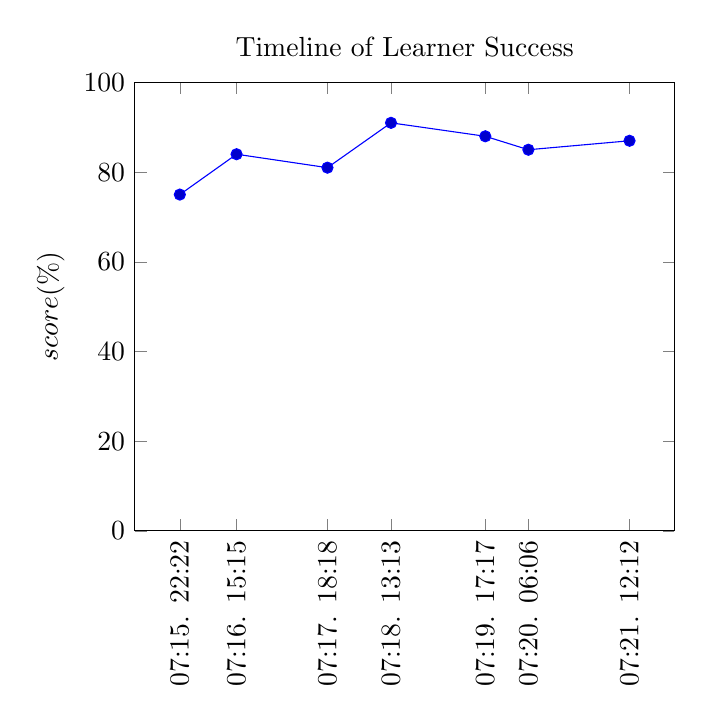
\begin{tikzpicture}
  \begin{axis}[
    title = Timeline of Learner Success,
    ylabel = $score(\%)$,
    ymin = 0,
    ymax = 100,
    date coordinates in=x,
    xtick=data,
    xticklabel style=
    {rotate=90,anchor=near xticklabel},
    xticklabel=\month:\day. \hour:\minute,]
    \addplot coordinates {
      (2018-07-15 22:22, 75.0)
      (2018-07-16 15:15, 84.0)
      (2018-07-17 18:18, 81.0)
      (2018-07-18 13:13, 91.0)
      (2018-07-19 17:17, 88.0)
      (2018-07-20 06:06, 85.0)
      (2018-07-21 12:12, 87.0)
    };
  \end{axis}
\end{tikzpicture}

\subsection{Prototype Improvement Suggestions}
Additional features may be implemented on top of this base
specification but they would require adding aditional values to each
subarray returned by the algorithm. These additional values can be
retrieved via (1) performing metadata lookup within or independently of the
algorithm (2) by utilizing additional xAPI statement paramters and/or (3) by
performing additional computations. The following examples assume the
metadata is contained within each statement available to the algorithm.
\begin{itemize}
\item A tooltip containing the name of an activity when hovering
  over a specific point on the chart
  \begin{itemize}
  \item this would require utilizing $\$.object.definition.name$
  \end{itemize}
\item A tooltip containing the device on which the activity was experienced
  \begin{itemize}
  \item this would require utilizing $\$.context.platform$
  \end{itemize}
\item A tooltip containing the instructor associated with a
  particular data point
  \begin{itemize}
  \item this would require utilizing $\$.context.instructor$
  \end{itemize}
\end{itemize}

\section{Which Assessment Questions are the Most Difficult}
As learners engage in activities supported by a learning ecosystem, they will
experience learning content as well as assessment content. Assessments
are designed to measure the effectiveness of learning content and help
assess knowledge gained. It is possible that certain assessment questions
do not accurately represent the concepts contained within learning
content and this may be indicated by a majority of learners getting
the question wrong. It is also possible that the question accurately
represents the learning content but is very difficult. The following
algorithm will identify these types of questions but will not be able to deduce
why learners answer them incorrectly.

\subsection{Ideal Statements}
In order to accurately determine which assessment questions are the
most dificult, there are a few requirements of the data produced by a
LRP. They are as follows:
\begin{itemize}
\item statements describing a learner answering a question must report
  if the learner got the question correct or incorrect via $\$.result.success$
\item if it is possible to get partial credit on a question, the amount
  of credit should be reported within the statement
  \begin{itemize}
  \item the credit earned by the learner should be reported within \\ $\$.result.score.raw$
  \item the minimum and maximum possible credit amount should be
    reported within $\$.result.score.min$ and $\$.result.score.max$
    respectively
  \end{itemize}
\item If it is possible to get partial credit on a question, it must
  still be reported if the learner reached the threshold of success
  via $\$.result.success$
\item Statements describing a learner answering a question should
  contain activities of the type $cmi.interaction$
\item activities must be uniquely and consistently identified across
  all statements
\item Statements describing a learner answering a question
  should\footnote{\label{verbIRI} it is possible to use another verb iri but if another is
    used, that will need to be accounted for in data retrieval} use
  the verb $http://adlnet.gov/expapi/verbs/answered$
\end{itemize}

\subsection{Input Data Retrieval}
How to query an LRS via a GET request to the Statements Resource via
curl. The following section contains the appropriate parameters with
example values as well as the curl command necessary for making the request.\footnote{\label{refMoreLink} See footnote 1.}\footnote{\label{refnoZ} See footnote 2.}\footnote{\label{refallTime} See footnote 3.}

\begin{lstlisting}[frame=single]
Verb = "verb=http://adlnet.gov/expapi/verbs/answered"

Since = "since=2018-07-20T12:08:47Z"

Until = "until=2018-07-21T12:08:47Z"

Base = "https://example.endpoint/statements?"

endpoint = Base + Verb + "&" + Since + "&" + Until

Auth = Hash generated from basic auth

S = curl -X GET -H "Authorization: Auth"
         -H "Content-Type: application/json"
         -H "X-Experience-API-Version: 1.0.3"
         Endpoint
\end{lstlisting}

\subsection{Statement Parameters to Utilize}

The statement parameter locations here are written in
\href{http://goessner.net/articles/JsonPath/}{JSONPath}. This notation
is also compatable with the xAPI Z notation due to the defined
hierarchy of components. Within the Z specifications, a variable name
will be used instead of the $\$$
\begin{itemize}
\item $\$.result.success$
\item $\$.object.id$
\end{itemize}

\subsection{2018 Pilot TLA Statement Problems}
The initial pilot test data supports this algorithm.
Given that the offical 2018 pilot test is scheduled to take place on July
27th, 2018, this section may require updates pending future data review.

\subsection{Summary}

\begin{enumerate}
\item Query an LRS via a \href{https://github.com/adlnet/xAPI-Spec/blob/master/xAPI-Communication.md#213-get-statements}{GET} request to the statements endpoint using the parameters verb, since and until
\item Filter the results to the set of statements where:
  \begin{itemize}
  \item $\$.result.success$ is false
  \end{itemize}
\item process the filtered data
  \begin{itemize}
  \item group by $\$.object.id$
  \item determine the count of each group
  \item create a collection of pairs = [$\$.object.id$, \#]
  \end{itemize}
\end{enumerate}

\subsection{Formal Specification}
\subsubsection{Basic Types}

$INCORRECT$ :== $\{false\}$

\subsubsection{System State}
\begin{schema}{MostDifficultAssessmentQuestions}
  Statements \\
  S_{all} : \finset_1 \\
  S_{incorrect},S_{grouped},S_{processed} : \finset \\
  \where
  S_{all} = statements \\
  S_{incorrect} \subseteq S_{all} \\
  S_{grouped} = \{groups : \seq_1 statement\} \\
  S_{processed} = \{pair : (id , \nat)\}
\end{schema}
\begin{itemize}
\item The set $S_{all}$ is a non-empty, finite set and is the
  component $statements$
\item The sets $S_{incorrect}$, $S_{grouped}$ and $S_{processed}$ are all finite sets
\item the set $S_{incorrect}$ is a subset of $S_{all}$ which may
  contain every value within $S_{all}$
\item the set $S_{grouped}$ is a finite set of objects $groups$ which
  are non-empty, finite sequences of the component $statement$
\item the set $S_{processed}$ is a finite set of pairs where each
  contains the component $id$ and a natural number
\end{itemize}
\subsubsection{Initial System State}

\begin{schema}{InitMostDifficultAssessmentQuestions}
  MostDifficultAssessmentQuestions \\
  \where
  S_{all} \not = \emptyset \\
  S_{incorrect} = \emptyset \\
  S_{grouped} = \emptyset \\
  S_{processed} = \emptyset
\end{schema}
\begin{itemize}
\item The set $S_{all}$ is a non-empty set
\item The sets $S_{incorrect}$ , $S_{grouped}$ and $S_{processed}$ are all initially empty
\end{itemize}

\subsubsection{Filter for Incorrect}

\begin{schema}{Incorrect}
  Statement \\
  incorrect : STATEMENT \pfun \finset \\
  s? : STATEMENT \\
  s! : \finset \\
  \where
  s? = statement \\
  s! = incorrect(s?) \\
  incorrect(s?) = \IF s?.result.success : INCORRECT \\\t4 \THEN s! =
  s? \\\t4 \ELSE s! = \emptyset
\end{schema}
\begin{itemize}
\item the schema $Incorrect$ introduces the function $incorrect$ which
  takes in the variable $s?$ and returns the variable $s!$
\item the variable $s?$ is the component $statement$
\item $s!$ is equal to $s?$ if $\$.result.success$ is of the type
  $INCORRECT$ otherwise $s!$ is an empty set
\end{itemize}

\begin{schema}{FilterForIncorrect}
  \Delta MostDifficultAssessmentQuestions \\
  Incorrect \\
  incorrects : \finset
  \where
  incorrects \subseteq S_{all} \\
  incorrects' = \{s : STATEMENT \,|\, incorrect(s) \not = \emptyset\} \\
  S_{incorrect}' = S_{incorrect} \cup incorrects'
\end{schema}
\begin{itemize}
\item the set $incorrects$ is a subset of $S_{all}$ which may contain
  every value within $S_{all}$
\item The set $incorrects'$ contains elements $s$ of type $STATEMENT$
  where $incorrect(s)$ is not an empty set
\item The updated set $S_{incorrect}'$ is the union of the previous
  state of $S_{incorrect}$ and $incorrects'$
\end{itemize}

\subsubsection{Processes Results}

\begin{schema}{GroupByActivityId}
  Statements \\
  g? : \finset \\
  g! : \finset \\
  group : \finset \fun \finset
  \where
  g? = statements \implies \{g : statement\} \\
  g! = group(g?) \\
  g! = \{groups : \seq_1 statement \,|\, \\ \t1
  \LET \seq_1 statement_{i}..statement_{j} == \seq_1 s_{i}..s_{j} @ \\\t1
  \forall s_{n} : s_{i}..s_{j} @ i \leq n \leq j @ s_{i}.object.id =
  s_{j}.object.id = s_{n}.object.id\} \\
\end{schema}
\begin{itemize}
\item The schema $GroupByActivityId$ introduces the function $group$
  which has the input of $g?$ and the output of $g!$
\item The input variable $g?$ is the component $statements$ which implies
  its a set of objects $g$ which are each a $statement$
\item the output variable $g!$ is a set of objects $groups$ which
  are each a non-empty, finite sequence of $statement$ where each
  member of the sequence $s_{i}..s_{j}$ has the same $\$.object.id$
\end{itemize}

\begin{schema}{CountPerGroup}
  Statement \\
  c? : \seq_1 statement \\
  c! : \nat \\
  count : \seq_1 statement \fun \nat
  \where
  c! = count(c?) \\
  c! \geq 1 \\
  count(c?) = \forall c_{n}? : \langle c?_{i}..c?_{j} \rangle @ i \leq n \leq j \land i
  = 0 @ \\\t3  \exists_1 \, c! : \nat @  \IF n = i \THEN c! = n + 1 \ELSE c!
  = j + 1

\end{schema}
\begin{itemize}
\item The schema $CountPerGroup$ introduces the function $count$
  which has the input of $c?$ and the output of $c!$
\item The input variable $c?$ is a non-empty, finite sequence in which each element is
  a $statement$
\item The function $count$ reads: for all elements $c?_{n}$ within the
  sequence $\langle c?_{i}..c?_{j} \rangle$, such that $n$ is greater than or
  equal to $i$ and less than or equal to $j$, $i$ is
  equal to zero and there exits a number $c!$ which is equal to $n +
  1$ (when $n = i \implies n = 0$) or equal to $n$
\end{itemize}

\begin{schema}{AggregateQuestionStatements}
  \Delta MostDifficultAssessmentQuestions \\
  FilterForIncorrect \\
  GroupByActivityId \\
  CountPerGroup \\
  grouped, processed : \finset \\
  \where
  grouped = \emptyset \\
  grouped' = group(S_{incorrect}) \\
  S_{grouped}' = S_{grouped} \cup grouped' \\
  processed \subseteq S_{grouped}' \\
  processed' = \{p : (id, \nat) \,|\, \\\t3 \LET
  \{\langle processed_{i}\rangle..\langle processed_{j}\rangle\} == \{g_{i}..g_{j}\} @ \\\t3
  i \leq n \leq j @ \forall g_{n} : g_{i}..g_{j} @ \exists \, p_{n} : p_{i}..p_{j} @ \\\t3
  first~p_{n} = head~g_{n}.object.id \, \land second~p_{n} =
  count(g_{n}) \\
  S_{processed}' = S_{processed} \cup processed'
\end{schema}
\begin{itemize}
\item The schema $AggregateQuestionStatements$ introduces the variables
  $grouped$ and $processed$
\item $grouped$ starts as an empty set but then becomes $grouped'$
  which is the output of applying the function $group$ to the set of statements
  $S_{incorrect}$ created by the opperation $FilterForIncorrect$
\item $grouped'$ is a set of sequences. The elements of those
  sequences are statements which all have the same
  $statement.object.id$

\item The set $S_{grouped}$ is updated to the set $S_{grouped}'$ which
  is the union of $S_{grouped}$ and $grouped'$
\item the variable $processed$ is a subset of $S_{grouped}'$ which can
  contain every value within $S_{grouped}'$
\item the variable $processed$ is updated to be the variable
  $processed'$ which is a set of objects $p$ which are ordered pairs
  of the component $id$ and a natural number. $p$ is defined as:
  \begin{itemize}
  \item for all sequences $g_{i}..g_{j}$ within the set $processed$,
    there exists an ordered pair $p_{n}$ such that:
    \begin{itemize}
    \item the first element of $p_{n}$ is equal to the $object.id$ of the first
      statement within the sequence $g_{n}$.
    \item The second element of $p_{n}$ is equal to the value returned
      when $g_{n}$ is passed to the function $count$.
    \end{itemize}
  \end{itemize}
\item The set $S_{processed}'$ is the union of the sets
  $S_{processed}$ and $processed'$
\end{itemize}

\subsubsection{Sequence of Operations}

$ProcessedQuestions \defs FilterForIncorrect \semi
AggregateQuestionStatements$

\begin{itemize}
\item The schema $ProcessedQuestions$ is the sequential composition
  of operation schemas $FilterForIncorrect$ and
  $AggregateQuestionStatements$
\item $FilterForIncorrect$ happens before $AggregateQuestionStatements$
\end{itemize}

\subsubsection{Return}

\begin{schema}{ReturnAggregate}
  \Xi MostDifficultAssessmentQuestions \\
  ProcessedQuestions \\
  S_{processed}! : \finset
  \where
  S_{processed}! = S_{processed}
\end{schema}
\begin{itemize}
\item The returned variable $S_{processed}!$ is equal to the current
  state of variable $S_{processed}$ after the operations
  $FilterForIncorrect$ and \\ $AggregateQuestionStatements$
\end{itemize}

\subsection{Pseudocode}

\begin{algorithm}[H]
  \SetAlgoLined
  \KwIn{$S_{all}$, $displayN$}
  \KwResult{$display''$}
  \emph{context = \{\}}\;
  \emph{display = []}\;
  \While{$S_{all} \not = \emptyset$}
  {\ForEach{$s \in S_{all}$}
    {\eIf{$s.result.success$ = $INCORRECT$}
      {\bf do \\
        $S_{incorrect}' \leftarrow s \cup S_{incorrect}$\;
        $S_{all}' \leftarrow S_{all} \setminus s$\;
        recur $S_{all}', S_{incorrect}'$\;}
      {\bf do \\
        $S_{all}' \leftarrow S_{all} \setminus s$\;
        recur $S_{all}'$}}}
  \While{$S_{incorrect}' \not = \emptyset$}
  {\ForEach{$si \in S_{incorrect}'$}
    {$id \leftarrow si.object.id$\;
      {\eIf{$id \notin context$}
        {\bf do \\
          $count = 1$\;
          $context' \leftarrow \{id : count\}$\;
          $S_{incorrect}' \leftarrow S_{incorrect} \setminus si$\;
          recur $context', S_{incorrect}'$\;}
        {\bf do \\
          $count' \leftarrow inc(context.id)$\;
          $context' \leftarrow \{id : count'\}$\;
          $S_{incorrect}' \leftarrow S_{incorrect} \setminus si$\;
          recur $context', S_{incorrect}'$\;}}}}
  \ForEach{$id \in context'$}
  {$IdToCount \leftarrow [id, context.id]$\;
    $display' \leftarrow display \cat IdToCount$\;
    {\bf recur} $display'$}
  \Return $display'' \leftarrow$ {\bf take(sortBySubArray($display'$), $displayN$)}
  \caption{Most Difficult Assessment Questions}
\end{algorithm}
\begin{itemize}
\item The Z schemas are used within this pseudocode
\item The return value display is an array of length display-n, where
  each element of display is an array of [$statement.object.id$, \#]
  where $\#$ representing the number of times $statement.object.id$
  appeared within $S_{incorrect}'$
\end{itemize}

\subsection{JSON Schema}

\begin{lstlisting}[style=json]
{"type":"array",
   "items":{"type":"array",
      "items":[{"type":"string"}, {"type":"number"}]}}
\end{lstlisting}

\subsection{Visualization Description}
The \textbf{Most Difficult Assessment Questions} visualization will be
a bar chart where the domain consists of $statement.object.id$ and the
range is a number greater than or equal to 1. Every subarray within
the array display will be a grouping within the bar chart. The
pseudocode specifies an input paramter display-n which controls the
length of the array display and therefor the number of groups contained within
the visualization.


\subsection{Visualization prototype}

\pgfplotstabletypeset[string type]

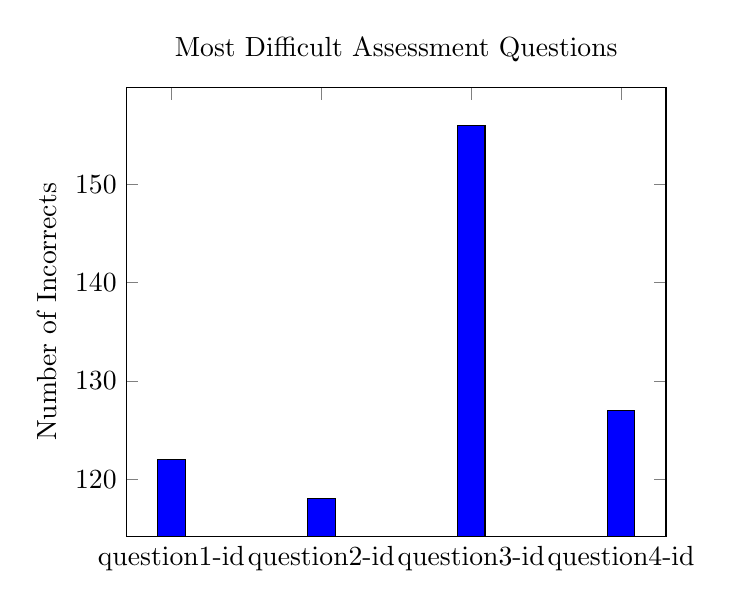
\begin{tikzpicture}
  \begin{axis}[
    title = Most Difficult Assessment Questions,
    ylabel = Number of Incorrects,
    symbolic x coords={question1-id,question2-id,question3-id,question4-id},
    xtick=data]
    \addplot[ybar,fill=blue] coordinates{
      (question1-id,122)
      (question2-id,118)
      (question3-id,156)
      (question4-id,127)
    };
  \end{axis}
\end{tikzpicture}

\subsection{Prototype Improvement Suggestions}
Additional features may be implemented on top of this base
specification but they would require adding aditional values to each
subarray returned by the algorithm. These additional values can be
retrieved via (1) performing metadata lookup within or independently
of the algorithm (2) by utilizing additional xAPI statement paramters
and/or (3) by performing additional computations. The following
examples assume the metadata is contained within each statement
available to the algorithm.

\begin{itemize}
\item Use the name of the activity for the x-axis label instead of
  its id.
  \begin{itemize}
  \item $\$.object.definition.name$
  \item grouping of statements should still happen by
    $\$.object.id$ to ensure an accurate count
  \end{itemize}
\item a tooltip containing contextual information about the question
  such as:
  \begin{itemize}
  \item The question text
    \begin{itemize}
    \item $\$.object.definition.description$
    \end{itemize}
  \item Interaction Type
    \begin{itemize}
    \item $\$.object.definition$ which contains interaction properties
    \end{itemize}
  \item Answer choices
    \begin{itemize}
    \item $\$.object.definition$ which contains interaction properties
    \end{itemize}
  \item Correct answer
    \begin{itemize}
    \item $\$.object.definition$ which contains interaction properties
    \end{itemize}
  \item Most popular incorrect answer
    \begin{itemize}
    \item This would require an extra step of processing and all
      statements would need to utilize interaction properties within
      $\$.object.definition$
    \end{itemize}
  \item average partial credit earned (if applicable)
    \begin{itemize}
    \item $\$.result.score.scaled$
    \item The one potential issue with using scaled score is the
      calculation of scaled is not stricly defined by the xAPI
      specification but is instead up to the authors of the LRP. This
      results in the inability to reliably compare scaled scores across LRPs.
    \item if $\$.result.score.raw$ , $\$.result.score.min$ and
      $\$.result.score.max$ are reported for all questions, it becomes
      possible to reliably compare scores across questions and LRPs.
    \end{itemize}
  \item average number of re-attempts
    \begin{itemize}
    \item this would require additional steps of processing so that
      $\$.actor$ is considered as well
    \item due to the problem of actor unification, ie the same
      person being identified differently across statements, this
      metric may not be accurate.
    \end{itemize}
  \item average time spent on the question
    \begin{itemize}
    \item $\$.result.duration$
    \item this would require additional steps of processing to
      extract the duration and average it.
    \end{itemize}
  \end{itemize}
\item a tooltip containing contextual information about the course
  and/or assessment the question was within
  \begin{itemize}
  \item the instructor for the course
    \begin{itemize}
    \item $\$.context.instructor$
    \end{itemize}
  \item competency associated with the question and/or course
    \begin{itemize}
    \item $\$.context.contextActivities$
    \end{itemize}
  \item metadata about the learning content associated with the
    question such as average time spent engaging with associated
    content before attempting the question.
  \item this would require additional steps of processing to
    retrieve metadata about the content and its usage.
    \begin{itemize}
    \item $\$.context.contextActivities$
    \end{itemize}
  \end{itemize}
\end{itemize}

\section{Rate of Completions}

As learners engage in activities supported by a learning ecosystem, they will build
up a history of learning experiences. When the digital resources of that learning ecosystem
adhere to a framework dedicated to supporting and understanding the
learner, such as the Total Learning Architecture (TLA), it becomes
possible to retell their learning story through data and data visualization. One important aspect of
that story is the rate of completion\footnote{\label{defOfCompletion}
  Completion can be defined by the presence of the verb completed or by the presence of
  $\$.result.completion$ set equal to true. In this algorithm,
  completion is defined by the presence of the verb completed
  regardless of $\$.result.completion$. This decision affects how
  statements are retrieved and filtered. In the case where completion
  is defined by $\$.result.completion$, the query to the LRS would not
  include the verb paramater and there would need to be a filtering
  process which looks for the presence of $\$.result.completion$ =
  true} of the various digital resources within the learning
ecosystem.
\subsection{Ideal Statements}

In order to accurately portray the rates of completion, there
are a few base requirements of the data produced by a Learning Record
Provider (LRP). They are as follows:
\begin{itemize}
\item statements describing a learner completing an activity
  should\footnote{\label{verbIRICompletion} See footnote 4}
  use the verb $http://adlnet.gov/expapi/verbs/completed$
\item statements describing a learner completing an activity should
  report if the learner was successful or not via
  $\$.result.success$
\item statement describing a learner completing a scored activity
  should report the learners score via $\$.result.score.raw$,
  $\$.result.score.min$ and $\$.result.score.max$
\item activites must be uniquely and consistently identified across
  all statements
\item The time at which a learner completed a learning activity must be recorded
  \begin{itemize}
  \item The timestamp should contain an appropriate level of specificity.
  \item ie. Year, Month, Day, Hour, Minute, Second, Timezone
  \end{itemize}
\item statements describing a learner completing an activity should
  report the amount of time taken to complete the activity via $\$.result.duration$
\end{itemize}

\subsection{Input Data Retrieval}

How to query an LRS via a GET request to the Statements Resource via
curl. The following section contains the appropriate parameters with
example values as well as the curl command necessary for making the
request.\footnote{\label{refMoreLink2} See footnote
  1.}\footnote{\label{refnoZ2} See footnote
  2.}\footnote{\label{refallTime2} See footnote 3.}

\begin{lstlisting}[frame=single]
Verb = "verb=http://adlnet.gov/expapi/verbs/completed"

Since = "since=2018-07-20T12:08:47Z"

Until = "until=2018-07-21T12:08:47Z"

Base = "https://example.endpoint/statements?"

endpoint = Base + Verb + "&" + Since + "&" + Until

Auth = Hash generated from basic auth

S = curl -X GET -H "Authorization: Auth"
         -H "Content-Type: application/json"
         -H "X-Experience-API-Version: 1.0.3"
         Endpoint
\end{lstlisting}

\subsection{Statement Parameters to Utilize}

The statement parameter locations here are written in
\href{http://goessner.net/articles/JsonPath/}{JSONPath}. This notation
is also compatable with the xAPI Z notation due to the defined
hierarchy of components. Within the Z specifications, a variable name
will be used instead of the $\$$
\begin{itemize}
\item $\$.timestamp$
\item $\$.object.id$
\end{itemize}

\subsection{2018 Pilot TLA Statement Problems}

The initial pilot test data supports the core requirements of this
algorithm but completion statements only reports completion scores via
$\$.result.scaled$ instead of $\$.result.score.raw$,
$\$.result.score.min$ and
$\$.result.score.max$.\footnote{\label{scaledScores} The one potential
  issue with using scaled score is the
  calculation of scaled is not stricly defined by the xAPI
  specification but is instead up to the authors of the LRP. This
  results in the inability to reliably compare scaled scores across
  LRPs. if $\$.result.score.raw$ , $\$.result.score.min$ and
  $\$.result.score.max$ are reported for all questions, it becomes
  possible to reliably compare scores across LRPs by generating a
  scaled score in a consistent way.} Given that the offical 2018 pilot
test is scheduled to take place on July 27th, 2018, this section may
require updates pending future data review.

\subsection{Summary}

\begin{enumerate}
  \item Query an LRS via a GET request to the statemetns endpoint
    using the paramters verb, since and until.
  \item group statements by their $\$.object.id$
  \item select time range unit for use within rate calculation. Will
    default to day.
  \item determine the amount of time between the first and last instance of a $\$.object.id$ (in seconds) and divide it by the time unit. ie if the unit is minute, you would divide by 60.
  \item calculate the rate by dividing the count of a group (2) by the number of time units covered by the statements (4) so that the rate is the number of completions per activity per time unit.
\end{enumerate}

\subsection{Formal Specification}

\subsubsection{Basic Types}

$TIMEUNIT$ :== $\{second\} | \{minute\} | \{hour\} | \{day\} |
\{week\} | \{month\} | \{year\}$

\subsubsection{System State}

\begin{schema}{RateOfCompletion}
  Statements \\
  S_{completions} : \finset_1 \\
  S_{grouped},S_{timeunit}, S_{processed} : \finset \\
  \where
  S_{completions} = statements \\
  S_{grouped} = \{byId : \seq_1 statement\} \\
  S_{withRate} = \{byGroup: (\seq_1 statement, \nat)\} \\
  S_{processed} = \{rate : (id , \nat, TIMEUNIT)\}
\end{schema}
\begin{itemize}
\item The set $S_{completions}$ is a non-empty, finite set and is the
  component $statements$ which contains the results of the query to
  the LRS.
\item The sets $S_{grouped}$, $S_{withRate}$ and $S_{processed}$ are all finite sets
\item the set $S_{grouped}$ is a finite set of objects $byId$ which
  are non-empty, finite sequences of the component $statement$
\item the set $S_{withRate}$ is a finite set of objects $byGroup$ which
  are ordered pairs of non-empty, finite sequences of the component $statement$ and a natural number
\item the set $S_{processed}$ is a finite set of objects $rate$ where each
  contains the component $id$, a natural number and the type $TIMEUNIT$
\end{itemize}

\subsubsection{Initial System State}

\begin{schema}{InitRateOfCompletion}
  RateOfCompletion \\
  T : TIMEUNIT
  \where
  S_{completions} \not = \emptyset \\
  S_{grouped} = \emptyset \\
  S_{withRate} = \emptyset \\
  S_{processed} = \emptyset \\
  T = \{day\}
\end{schema}
\begin{itemize}
\item The set $S_{completions}$ is a non-empty set which contains the results of the GET request(s) to the LRS
\item The sets $S_{grouped}$ , $S_{withRate}$ and $S_{processed}$ are
  all initially empty
\item the variable T has the type $TIMEUNIT$ and the value $\{day\}$
\end{itemize}

\subsubsection{Calculate Rate}

\begin{schema}{IsoToUnix}
  convert : \finset_1 \fun \nat\#1 \\
  c? : \finset_1 \\
  c! : \nat\#1
  \where
  c! = convert(c?)
\end{schema}
\begin{itemize}
  \item The schema $IsoToUnix$ introduces the function $convert$ which
    takes in a finit set of one thing (a timestamp) and converts it to
    a single natural number.
  \item the purpose of this function is to convert an ISO 8601
    timestamp to the Unix epoch. The concrete definition of the conversion
    is outside the scope of this document
    \begin{itemize}
      \item The Unix epoch is the number of seconds that have elapsed
        since January 1, 1970 (midnight UTC/GMT), not counting leap seconds.
    \end{itemize}
  \end{itemize}

\begin{schema}{CalcRateByUnit}
  Statement \\
  IsoToUnix \\
  CountPerGroup \\
  unit? : TIMEUNIT \\
  s?,s! : \finset \\
  r : \nat \\
  rate : (\finset, TIMEUNIT) \fun \finset
  \where
  unit? \, = \,\{second\} \implies 1 \lor \{minute\} \implies 60
  \lor \{hour\} \implies 3600 \,\lor \\\t2 \{day\} \implies 86400 \lor
  \{week\} \implies 604800 \,\lor \\\t2 \{month\} \implies 2629743
  \lor \{year\} \implies 31556926 \\
  s? = \{g : seq_1 statement\} \\
  s! = rate(s?, unit?) \\
  s! = \{s : (g, r) \,|\, \forall g_{n}: g_{i}..g_{j} @ i \leq n \leq j @
  \exists \, s_{n} : (g_{n}, r_{n}) @ \\\t1
  r_{n} = count(g_{n}) \div ((convert(last~g_{n}.timestamp) - convert(head~g_{n}.timestamp)) \div unit?)\}
\end{schema}
\begin{itemize}
\item The schema $CalcRateByUnit$ introduces the function $rate$ where
  the input $s?$ is a set of objects $g$ which are each a non-empty,
  finite sequence of statements and the input $unit?$ represents a
  unit of time.
\item for every $g_{n}$ within the range $g_{i}..g_{j}$, there exists an associated object $s_{n}$ which is an orderd pair of $(g_{n}, r_{n})$ where $r_{n}$ is equal to the number of items within $g_{n}$ divided by the number of $unit?$s within the time range of $last~g_{n}.timestamp-head~g_{n}.timestamp$
\item the output of the function $rate$ is $s!$, the set of all $s_{n}$
\end{itemize}
$\\\\\\\\\\\\\\\\\\\\\\\\\\$ %%% keep header with z-schema
\subsubsection{Processes Results}
\begin{schema}{AggergateCompletionStatements}
  \Delta RateOfCompletion \\
  GroupByActivityId \\
  CalcRateByUnit \\
  grouped,processed,withRate : \finset \\
  r : \nat \\
  T? : TIMEUNIT
  \where
  T? = \{day\} \\
  grouped = \emptyset \\
  grouped' = group(S_{completions}) \\
  S_{grouped}' = S_{grouped} \cup grouped' \\
  withRate \subseteq S_{grouped}' \\
  withRate' = rate(withRate, T?) \\
  S_{withRate}' = withRate' \cup S_{withRate} \\
  processed \subseteq S_{withRate}' \\
  processed' = \{p: (id, r, T?) \,|\,
  \\\t3 \LET \{processed_{i}..processed_{j}\} == \{b_{i}..b_{j}\} @ \\\t3
  \forall b_{n} : b_{i}..b_{j} @ i \leq n \leq j @
  \exists \, p_{n} : (id_{n}, r_{n}, T?) @  \\\t3
  id_{n} = (head~(first~b_{n})).object.id \, \land \, \\\t3
  r_{n} = (second~b_{n})\} \\
  S_{processed}' = processed' \cup S_{processed}
\end{schema}

\begin{itemize}
\item The schema $AggergateCompletionStatements$ outlines how to calculate
  the rate of completion per $\$.object.id$ per $second|minute|hour|day|week|month|year$
  \begin{enumerate}
  \item $S_{grouped}'$ is the result of grouping the statements within $S_{completions}$ by their $\$.object.id$
  \item The groups from (1) are passed to the function $rate$ with the
    variable $T?$ which controls the unit of time, ie per day vs per week
  \item the result of (2) is then processed to create a triplet of
    $\$.object.id$, rate, unit of time for all unique $\$.object.id$
    within $S_{completions}$
\end{enumerate}
\end{itemize}

\subsubsection{Return}

\begin{schema}{ReturnAggergateCompletionStatements}
  \Xi RateOfCompletion \\
  AggergateCompletionStatements \\
  S_{processed}! : \finset
  \where
  S_{processed}! = S_{processed}
\end{schema}
\begin{itemize}
  \item The return value $S_{processed}!$ is equal to $S_{processed}$ after the operation described by $AggergateCompletionStatements$
\end{itemize}

\subsection{Pseudocode}

\begin{algorithm}[H]
  \SetAlgoLined
  \KwIn{$S_{completed}$, $timeUnit$}
  \KwResult{$ratePerObjTu'$}
  \emph{context = \{\}}\;
  \emph {ratePerObjTu = []}\;
  \While{$S_{completion} \not = \emptyset$}
  {\ForEach{$s \in S_{completion}$}
    {$id \leftarrow s.object.id$\;
      $ts \leftarrow convert(s.timestamp)$\;
      \eIf{$id \notin context$}
      {\bf do \\
        $times = [ts]$\;
        $context' \leftarrow \{id : times \}$\;
        $S_{completion}' \leftarrow S_{completion} \setminus s$\;
        recur $context', S_{completion}'$\;}
      {\bf do \\
        $times' \leftarrow context.id \cat ts$\;
        $context' \leftarrow \{id : times'\}$\;
        $S_{completion}' \leftarrow S_{completion} \setminus s$\;
        recur $context', S_{completion}'$\;}}}
  \ForEach {$k \in context'$}
  {$allTs \leftarrow context'.k$\;
    $totalDuration \leftarrow max(allTs) - min(allTs)$\;
    $totalCount \leftarrow count(allTs)$\;
    $rate \leftarrow totalCount \div (totalDuration \div timeUnit)$\;
    $subVec = [k, rate, timeUnit]$\;
    $ratePerObjTu' \leftarrow ratePerObjTu \cat subVec$\;
    {\bf recur} $ratePerObjTu'$\;}
 \Return $ratePerObjTu'$
  \caption{Rate of Completions}
\end{algorithm}
\begin{itemize}
\item Values from Z schemas are used within this pseudocode
\item the result of the algorithm is an array of arrays where each
  subarray contains a $statement.object.id$, the $rate$ and the
  $timeUnit$ used to calculate $rate$.
\end{itemize}
$\\$ %% header with text
\subsection{JSON Schema}

\begin{lstlisting}[style=json]
{"type":"array",
   "items":{"type":"array",
      "items":[{"type":"string"}, {"type":"number"}, {"type":"string"}]}}
\end{lstlisting}

\subsection{Visualization Description}

The \textbf{Rate of Completions} visualization will be
a bar chart where the domain consists of $statement.object.id$ and the
range is a number greater than 0 (the rate of completions for that
$statement.object.id$). Every subarray within the array $ratePerObjTu$
will be a grouping within the bar chart. The pseudocode specifies an
input paramter $timeUnit$ which controls the calculation of the rate
(range of the visualization). $timeUnit$ could be per minute, per day,
per week, etc.

\subsection{Visualization prototype}

\pgfplotstabletypeset[string type]

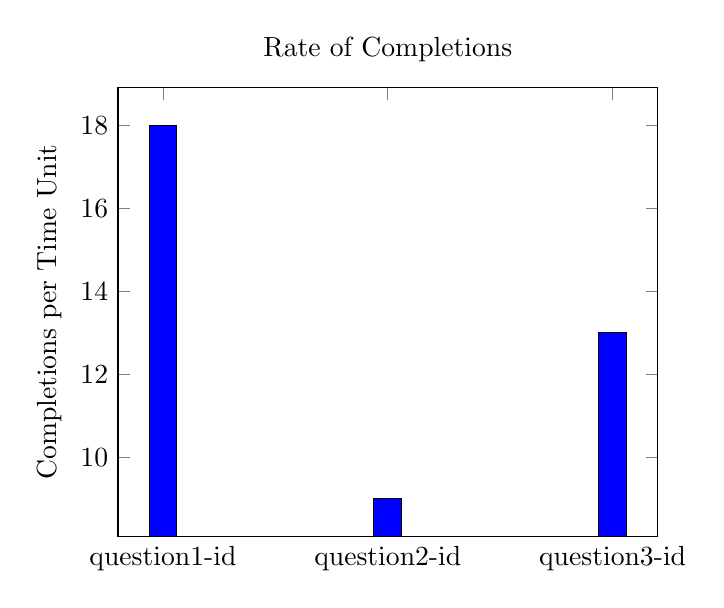
\begin{tikzpicture}
  \begin{axis}[
    title = Rate of Completions,
    ylabel = Completions per Time Unit,
    symbolic x coords={question1-id,question2-id,question3-id},
    xtick=data]
    \addplot[ybar,fill=blue] coordinates{
      (question1-id,18)
      (question2-id,9)
      (question3-id,13)
    };
  \end{axis}
\end{tikzpicture}

\subsection{Prototype Improvement Suggestions}
Additional features may be implemented on top of this base
specification but they would require adding aditional values to each
subarray returned by the algorithm. These additional values can be
retrieved via (1) performing metadata lookup within or independently of the
algorithm (2) by utilizing additional xAPI statement paramters and/or (3) by
performing additional computations. The following examples assume the
metadata is contained within each statement available to the algorithm.

\begin{itemize}
\item use $statement.object.definition.name$ instead of
  $statement.object.id$ for x axis label
\item populate a tooltip with the people who have completed the
  activity. This could also include the number of times they have
  completed it.
\item populate a tooltip with the breakdown of which devices or platforms the
  activity was completed on. This would require the device type or platform to be
  reported within $statement.context.platform$
\item populate a tooltip with the breakdown of percentage successful
  for all completions of the activty. This would require
  $statement.result.success$
\item populate a tooltip with the breakdown of scores earned (if
  appliciable) for the completions. This would require
  $statement.result.score.raw$, $statement.result.score.min$ and
  $statement.result.score.max$
\item populate a tooltip with the competency assocaited with the
  completed activities. The competency should be reported
  via $statement.context.contextActivities$
\item populate a tooltip with the average duration spent to reach
  completions. This would require $statement.result.duration$ to be reported.
\end{itemize}

\section{How Often are Recommendations Followed}

As learners engage in activities supported by a learning ecosystem, they will build
up a history of learning experiences. When the digital resources of that learning ecosystem
adhere to a framework dedicated to supporting and understanding the
learner, such as the Total Learning Architecture (TLA), it becomes
possible to retell their learning story through data and data
visualization. One important aspect of that story is the
recommendations provided to the learner and whether or not the learner
follows those recommendations.

\subsection{Ideal Statements}

In order to accurately determine if a learner is following
recommendations, there are a few requirements of the data produced by
a LRP and the recommender itself. They are as follows:

\begin{itemize}
\item Every time the recommender makes a recommendation, a statement
  should be produced which uses the verb
  $https://w3id.org/xapi/dod-isd/verbs/recommended$\footnote{\label{RecommendedIRI}
  See footnote 4} and has the
  recommended piece of content as the object.
  \begin{itemize}
    \item the content should be uniquely and consistently identified
      across all statements.
    \end{itemize}
\item When a learner launches recommended content, the resulting
  launched statement should use the verb
  $http://adlnet.gov/expapi/verbs/launched$\footnote{\label{LaunchedIRI}
  See footnote 4} and contain a refrence to the recommened content statement within
  $\$.context.statement$
  \begin{itemize}
    \item Launching of content should use the above IRI regardless of
      why the content was launched
    \item If it not possible to refrence the exact recommended content
      statement, the launch statement should have some indication that
      it was the result of a recommendation.\footnote{\label{Recommendations} It is
    possible to determine if recommendations are followed (with some
    level of error) without this explicit linking of launched to
    recommended but this severly complicates the algorithm. In this
    case, in order to optmize for accuracy, the algorithm would need
    to consider the actor and their general activity within a session,
    the object of both launched and recommended statements generated
    within the session, the time lapse between recommendations and
    launches with a predefined lapse value which determines if a
    launch was close enough in time to a recommendation to be
    considered a result of the recommendation. An additonal constraint
    on the above case is the recommendation statements should contain
    a reference to to the person recieving the recommendation,
    otherwise determining the 1:1 relationships between recommendations and
    launches requires aditional complexity and will still not be 100\%
    accurate due to the reliance on the time lapse value.}
  \end{itemize}
\end{itemize}

\subsection{Input Data Retrieval}

How to query an LRS via a GET request to the Statements Resource via
curl.\footnote{\label{refMoreLink2} footnote 1 applies to both S1
  and S2.}\footnote{\label{refnoZ2} See footnote
  2.}\footnote{\label{refallTime2} See footnote 3.}

\begin{lstlisting}[frame=single]
R = "verb=https://w3id.org/xapi/dod-isd/verbs/recommended"
L = "verb=http://adlnet.gov/expapi/verbs/launched"

Since = "since=2018-07-20T12:08:47Z"
Until = "until=2018-07-21T12:08:47Z"

Base = "https://example.endpoint/statements?"

endpoint1 = Base + R + "&" + Since + "&" + Until
endpoint2 = Base + L + "&" + Since + "&" + Until

Auth = Hash generated from basic auth

SR = curl -X GET -H "Authorization: Auth"
         -H "Content-Type: application/json"
         -H "X-Experience-API-Version: 1.0.3"
         endpoint1
SL = curl -X GET -H "Authorization: Auth"
         -H "Content-Type: application/json"
         -H "X-Experience-API-Version: 1.0.3"
         endpoint2

S = SR + SL
\end{lstlisting}

\subsection{Statement Parameters to Utilize}

The statement parameter locations here are written in
\href{http://goessner.net/articles/JsonPath/}{JSONPath}. This notation
is also compatable with the xAPI Z notation due to the defined
hierarchy of components. Within the Z specifications, a variable name
will be used instead of the $\$$
\begin{itemize}
\item $\$.verb.id$
\item $\$.context.statement$
\end{itemize}

\subsection{2018 Pilot TLA Statement Problems}
At the time of writing this document, launched statements do not
include a statement reference or any indication of a connection
between recommendations and launches. The authors of this document do
not have access to the LRS containing the recommended statements and
thus can not draw any conclusions about any issues which may be
present within those statements or any aspects of those statements
which may correlate them to launch statements. The following algorithm
is going to assume that the input set of statements follow the
guidlines outlined in section 5.1 as the additional algorithmic
considerations brought on by non ideal statements, as specified within
footnote 16, result in an algoirthm which is not optimal for near real
time visualizations.

\subsection{Summary}
\begin{enumerate}
  \item Query an LRS via a GET request to the statements endpoint
    using the paramters verb, since and until to gather all statements
    with the verb $http://adlnet.gov/expapi/verbs/launched$.
  \item Query an LRS via a GET request to the statements endpoint
    using the paramters verb, since and until to gather all statements
    with the verb $https://w3id.org/xapi/dod-isd/verbs/recommended$.
    \footnote{\label{sameSession} If since and until are specified,
      they should be the same in both requests.}
  \item seperate the collection of launched statements (1) into a
    collection of those which were the result of a recommendation and
    those which were not.
  \item Group all collections of statements by a $TIMEUNIT$
  \item Take the count of all groups of statements from (4)
    \begin{itemize}
    \item Recommended statements per $TIMEUNIT$
    \item Launches due to recommendations per $TIMEUNIT$
    \item Launches not due to recommendations per $TIMEUNIT$
    \end{itemize}
  \item Calculate summary statistics for the overall time range and
    per $TIMEUNIT$
    \begin{itemize}
    \item Divide launches due to recommendations by the total number of
      launches to determine the percentage of launches due to
      recommendations
    \item Divide launches due to recommendations by the total number
      of recommendations to determine the percentage of
      recommendations which are followed.
    \end{itemize}
\end{enumerate}

\subsection{Formal Specification}

\subsubsection{System State}

\begin{schema}{FollowedRecommendations}
  Statements \\
  S_{recommended},S_{launched} : \finset_1 \\
  %%S_{processed}, S_{followed}, S_{independent}, S_{grouped} : \finset \\
  %%G_{followed}, G_{independent}, G_{recommended} : seq \, statement \\
  %%N_{launches}, N_{recommendations}, N_{followed}, P_{followed},
  %%P_{dueto} : \nat \\
  T : TIMEUNIT
  \where
  S_{recommended} = statements \\
  S_{launched} = statements \\
  %%S_{followed} \subseteq S_{launched} \\
  %%S_{independent} \subseteq S_{launched} \\
  %%S_{launched} = S_{followed} \cup S_{independent} \\
  %%\emptyset = S_{followed} \cap S_{independent} \\
  %S_{grouped} = \{byTimeUnit : (G_{followed}, G_{independent}, G_{recommended})\} \\
  %S_{processed} = \{summary : (N_{launches}, N_{recommendations},
  %N_{followed}, \\\t6 P_{followed}, P_{dueto}, statement.timestamp,
  %TIMEUNIT)\}
\end{schema}

\begin{itemize}
\item $S_{recommended}, S_{launched}$ are both non-empty, finite sets.
  \begin{itemize}
  \item $S_{recommended}$ and $S_{launched}$ contain
    the results of querying an LRS for recommended and launched
    statements respectively.
  \end{itemize}
\item $S_{followed}$, $S_{independent}$, $S_{grouped}$ and $S_{processed}$ are each finite
  sets.
  \begin{itemize}
    \item $S_{followed}$ and $S_{independent}$ are both subsets of
      $S_{launched}$.
    \item the union of $S_{followed}$ and $S_{independent}$ is the set
      $S_{launched}$
    \item $S_{followed}$ and $S_{independent}$ have no overlap
    \item $S_{grouped}$ is a set of objects $byTimeUnit$ which are
      each a collection of $G_{followed}, G_{independent},
      G_{recommended}$
    \item $S_{processed}$ is a set of objects $summary$ which are each a
      collection of $N_{launches}$, $N_{recommendations}$,
      $N_{followed}$, $P_{followed}$, $P_{dueto}$,
      $statement.timestamp$ and $TIMEUNIT$.
    \end{itemize}
\item $G_{followed}$, $G_{independent}$ and $G_{recommended}$ are each a
  finite sequence of statements.
\item $N_{launches}, N_{recommendations}, N_{followed}, P_{followed},
  P_{dueto}$ are all natural numbers
\end{itemize}

\subsubsection{Initial System State}

\begin{schema}{InitFollowedRecommendations}
  FollowedRecommendations \\
  T : TIMEUNIT
  \where
  S_{recommended} \not = \emptyset \\
  S_{launched} \not = \emptyset \\
  S_{processed} = \emptyset \\
 % S_{followed} = \emptyset \\
 % S_{independent} = \emptyset \\
 % S_{grouped} = \emptyset \\
 % G_{followed} = \emptyset \\
 % G_{independent} = \emptyset \\
 % G_{recommended} = \emptyset \\
 % N_{launches} = 0 \\
 % N_{recommendations} = 0 \\
 % N_{followed} = 0 \\
 % P_{followed} = 0 \\
 % P_{dueto} = 0 \\
 % T = \{day\}
\end{schema}

\begin{itemize}
  \item $S_{recommended}$ and $S_{launched}$ are initially not empty
    sets
  \item all other sets are initially empty
  \item all numbers are initially zero
  \item the default $TIMEUNIT$ is set to day
\end{itemize}


\subsubsection{Group by Timestamp}

\begin{schema}{SortByTimestamp}
  Statement \\
  IsoToUnix \\
  orderByTimestamp : \finset_1 \fun seq_1 \\
  o? : \finset_1 \\
  o! : seq_1 statement
  \where
  o? = \{o : statement\} \\
  o! = orderByTimestamp(o?) \\
  o! = \langle o_{i}..o_{j} \rangle @ \forall o_{n} : o_{i}..o_{j} @
  o_{n} : STATEMENT \land i \leq n \leq j @ \\\t3
  convert(o_{i}.timestamp) \leq convert(o_{n}.timestamp) \leq
  convert(o_{j}.timestamp)
\end{schema}

\begin{schema}{WithinRange}
  withinRange : (\nat, \nat, \nat, TIMEUNIT) \fun \finset_1\#1 \\
  in?, start?, state? : \nat \\
  unit? : TIMEUNIT \\
  out! : \{TRUE\} \lor \{FALSE\}
  \where
  unit? \, = \,\{second\} \implies 1 \lor \{minute\} \implies 60
  \lor \{hour\} \implies 3600 \,\lor \\\t2 \{day\} \implies 86400 \lor
  \{week\} \implies 604800 \,\lor \\\t2 \{month\} \implies 2629743
  \lor \{year\} \implies 31556926 \\

  out! = withinRange(in?, start?, state?, unit?) \\
  withinRange(in?, start?, state?, unit?) = \\\t3 \IF in? \leq
  start? + ((state? + 1) * unit?) \\\t4 \THEN out! = \{TRUE\} \\\t4 \ELSE
  out! = \{FALSE\} \\
\end{schema}

\begin{schema}{GroupByTimeUnit}
  Statement \\
  IsoToUnix \\
  WithinRange \\
  groupByTimeUnit : (\seq_1, \nat, TIMEUNIT) \fun \seq_1 \\
  g?,g! : \seq_1 \\
  t_{start}? : \nat
  \where
  g? = \langle g?_{i}..g?_{j} \rangle @ \forall g?_{n} :
  g?_{i}..g?_{j} @ i \leq n \leq j @ g?_{n} = statement \\

  g! = groupByTimeUnit(g?, t_{start}? state?, unit?) \\
  g! = \langle g : seq \,|\, \forall g?_{n} :
  g?_{i}..g?_{j} @
  \exists_1 \langle g_{r} \rangle : \langle g_{q} \rangle
  .. \langle g_{s} \rangle @ q \leq r \leq s \land r = state? @
  \\\t3 \IF withinRange(g?_{n}, t_{start}, r, unit?) =
  \{TRUE\} \\\t4 \THEN g?_{n} \inseq \langle g_{r} \rangle \\\t4 \ELSE
  \IF \forall g_{n}? : g_{i}?..g_{j}? @ withinRange(g?_{n}, t_{start}, r, unit?) =
  \{FALSE\} \\\t5 \THEN \langle g_{r} \rangle = \langle \rangle \land
  groupByTimeUnit(g?, t_{start}? (r + 1), unit?)\rangle
\end{schema}

\subsubsection{Processes Results}

\begin{schema}{OrderStatements}
  \Delta FollowedRecommendations \\
  SortByTimestamp \\
  orderedL, orderedR : seq_1 \\
  t_{start} : \nat
  \where
  orderedL = orderByTimestamp(S_{launched}) \\
  orderedR = orderByTimestamp(S_{recommended}) \\
  t_{start} = convert((head~orderedL).timestamp) \\
\end{schema}

\begin{schema}{GroupByTime}
  \Delta FollowedRecommendations \\
  OrderStatements \\
  GroupByTimeUnit \\
  CountPerGroup
  \where
  unit? = \{day\} \\
  grouped_{launched} = groupByTimeUnit(orderedL, t_{start}, 0, unit?) \\
  grouped_{recommended} = groupByTimeUnit(orderedR, t_{start}, 0,
  unit?) \\
  count(grouped_{launched}) = count(grouped_{recommended})
\end{schema}

\begin{schema}{OnlyRecommendedLaunches}
  \Delta FollowedRecommendations \\
  GroupByTime \\
  CountPerGroup
  \where
  onlyRecommended = \langle o : seq \,|\, \LET grouped_{launched}==gl
  \implies \\\t5 \langle \langle gl_{i} \rangle..\langle gl_{j}
  \rangle \rangle \implies \langle \langle gl_{ii}..gl_{ij}
  \rangle..\langle gl_{ji}..gl_{jj}\rangle\rangle @ \\\t5
  \forall \langle gl_{n} \rangle : \langle gl_{i} \rangle..\langle
  gl_{j} \rangle @ \exists_1 \langle o_{n} \rangle : \langle o_{i}
  \rangle..\langle o_{j} \rangle \implies \langle \langle o_{ii}..o_{ij} \rangle..\langle
  o_{ji}..o_{jj}\rangle\rangle @ \\\t5 ((\forall o_{in} : o_{ii}..o_{ij} @
  o_{in}.context.statement \not = \emptyset \land o_{in} \inseq
  gl_{i}) \land \\\t5 (\forall o_{jn} : o_{ji}..o_{jj} @
  o_{jn}.context.statement \not = \emptyset \land o_{jn} \inseq
  gl_{j})) \lor \\\t5 \langle o_{n} \rangle = \langle \rangle \rangle \\
  count(onlyRecommended) = count(grouped_{launched}) = count(grouped_{recommended})

\end{schema}

\begin{schema}{GetCounts}
  \Delta FollowedRecommendations
  CountPerGroup \\
  OrderStatements \\
  GroupByTime \\
  OnlyRecommendedLaunches \\
  \where
  cPerGroup_{launched} = \langle c : \nat \,|\, \LET grouped_{launched}==gl \implies
  \langle \langle gl_{i} \rangle..\langle gl_{j} \rangle \rangle @ \\\t5
  \forall \langle gl_{n} \rangle : \langle gl_{i} \rangle..\langle gl_{j} \rangle @
  \exists_1 c_{n} : \nat @ \\\t5 \IF gl_{n} = \langle \rangle \\\t6 \THEN c_{n} =
  0 \\\t6 \ELSE c_{n} = count(\langle gl_{n} \rangle)
  \rangle \\
  cPerGroup_{recommended} = \langle c : \nat \,|\, \LET grouped_{recommended}==gr \implies
  \langle \langle gr_{i} \rangle..\langle gr_{j} \rangle \rangle @ \\\t6
  \forall \langle gr_{n} \rangle : \langle gr_{i} \rangle..\langle gr_{j} \rangle @
  \exists_1 c_{n} : \nat @ \\\t5 \IF gr_{n} = \langle \rangle \\\t6 \THEN c_{n} =
  0 \\\t6 \ELSE c_{n} = count(\langle gr_{n} \rangle)
  \rangle \\
  cPerGroup_{followed} = \langle c : \nat \,|\, \LET
  onlyRecommended==or \implies \langle \langle or_{i} \rangle..\langle or_{j} \rangle \rangle @ \\\t5
  \forall \langle or_{n} \rangle : \langle or_{i} \rangle..\langle or_{j} \rangle @
  \exists_1 c_{n} : \nat @ \\\t5 \IF or_{n} = \langle \rangle \\\t6 \THEN c_{n} =
  0 \\\t6 \ELSE c_{n} = count(\langle or_{n} \rangle) \rangle \\
  count(cPerGroup_{launched}) = count(cPerGroup_{followed}) = count(cPerGroup_{recommended})
\end{schema}

\begin{schema}{CombineSequences}
  \Delta FollowedRecommendations \\
  GetCounts \\
  GroupByTime
  \where
  combined = \langle c : (tr_{start}, tr_{end}, N_{launched},
  N_{recommended}, N_{followed}, P_{followed}, P_{dueto}) \,|\, \\\t3
  \LET grouped_{launched}==gl \implies \langle \langle gl_{i}
  \rangle..\langle gl_{j} \rangle \rangle \\\t3\:\:\:\:\:\:\:
  cPerGroup_{launched}==cl \implies \langle cl_{i}..cl_{j} \rangle \\\t3\:\:\:\:\:\:\:
  cPerGroup_{recommended}==cr \implies \langle cr_{i}..cr_{j} \rangle \\\t3\:\:\:\:\:\:\:
  cPerGroup_{followed}==cf \implies \langle cf_{i}..cf_{j} \rangle \\\t3\:\:\:\:\:\:\:
  @ \forall \langle gl_{n} \rangle : \langle gl_{i} \rangle..\langle
  gl_{j} \rangle @ i \leq n \leq j @
  \\\t3\:\:\:\:\:\:\: \exists_1 \, c_{n} : (tr_{startn}, tr_{endn},
  cl_{n}, cr_{n}, cf_{n}, P_{followedn}, P_{dueton}) @
  \\\t3\:\:\:\:\:\:\: tr_{startn} = (head~gl_{n}).timestamp
  \\\t3\:\:\:\:\:\:\: tr_{endn} = (last!gl_{n}).timestamp
  \\\t3\:\:\:\:\:\:\: P_{followedn} = cf_{n} \div cr_{n}
  \\\t3\:\:\:\:\:\:\: P_{dueton} = cf_{n} \div cl_{n} \rangle
\end{schema}

\subsubsection{Return}
\subsection{Pseudocode}
\subsection{JSON Schema}
\subsection{Visualization Description}
\subsection{Visualization prototype}
\subsection{Prototype Improvement Suggestions}

\section{Appendex A: Visualization Examplars}
Appendex A includes a typology of data visualizations which may be supported by the DAVE Framework.
These visualizations can either be one to one or one to many in regards to the algorithms defined within this document.
Future iterations of this document will increasingly include these typologies within the domain-question template exemplars.

\begin{figure*}[h]
  \centering
  \begin{floatrow}[3]
    \ffigbox[\FBwidth*3/2]
    {\caption{Line Chart}
        \label{fig1}}
    {\begin{tikzpicture}
        \begin{axis}
          \addplot+[sharp plot] coordinates
          {(0,0) (1,2) (2,3)};
        \end{axis}
      \end{tikzpicture}}
    \ffigbox[\FBwidth*3/2]
    {\caption {Line with Error}
      \label{fig2}}
      {\begin{tikzpicture}
          \begin{axis}
            \addplot+[error bars/.cd,x dir=both,x explicit]
            coordinates {
              (0,0)   +- (0.1,0)
              (0.5,1) +- (0.4,0.2)
              (1,2)
              (2,5)   +- (1,0.1)
            };
          \end{axis}
        \end{tikzpicture}}
    \end{floatrow}
\end{figure*}

\begin{figure*}[h]
  \centering
  \begin{floatrow}[3]
    \ffigbox[\FBwidth*4/3]
    {\caption{Spline Chart}
      \label{fig3}}
    {\begin{tikzpicture}
        \begin{axis}[nodes near coords={(\coordindex)}]
          \addplot[mark=*, patch,mesh, patch type=cubic spline]
          coordinates {
            % left, right, left middle, right middle
            (-1,-1)
            (1,1)
            (-1/3,{(-1/3)^3})
            (1/3,{(1/3)^3})};
        \end{axis}
      \end{tikzpicture}}
  \ffigbox[\FBwidth*5/4]
  {\caption{Grouped Line Charts}\label{Fig4}}
  {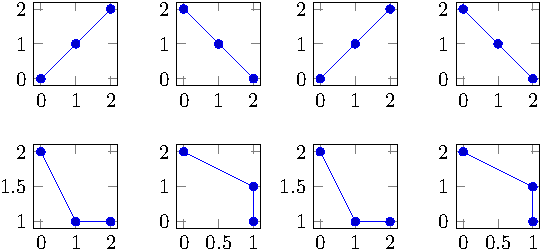
\includegraphics[page=1]{/Users/will/projects/dave/resources/plots/multiple_line.pdf}}
  \end{floatrow}
\end{figure*}

\begin{figure*}[h]
  \centering
  \begin{floatrow}[3]
    \ffigbox[\FBwidth*4/3][\FBheight+2cm]
    {\caption{Quiver Chart}\label{Fig5}}
    {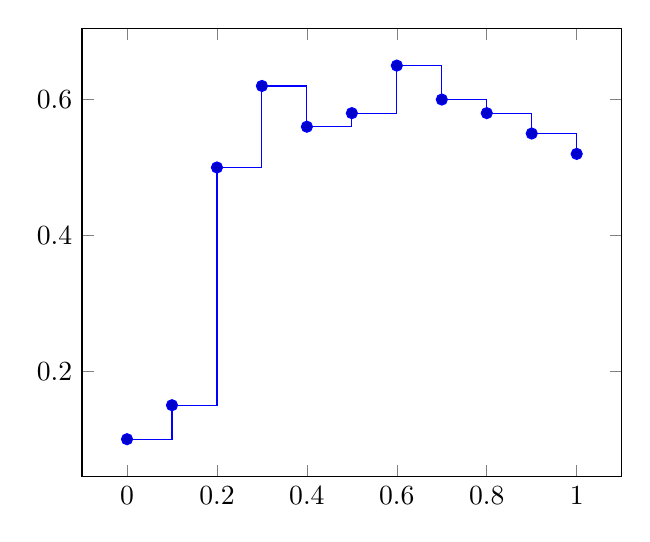
\begin{tikzpicture}
        \begin{axis}
          \addplot+[const plot]
          coordinates
          {(0,0.1)    (0.1,0.15)  (0.2,0.5)   (0.3,0.62)
            (0.4,0.56) (0.5,0.58)  (0.6,0.65)  (0.7,0.6)
            (0.8,0.58) (0.9,0.55)  (1,0.52)};
        \end{axis}
      \end{tikzpicture}}%
    \ffigbox[\FBwidth*4/3]
    {\caption{Histogram}\label{fig6}}
    {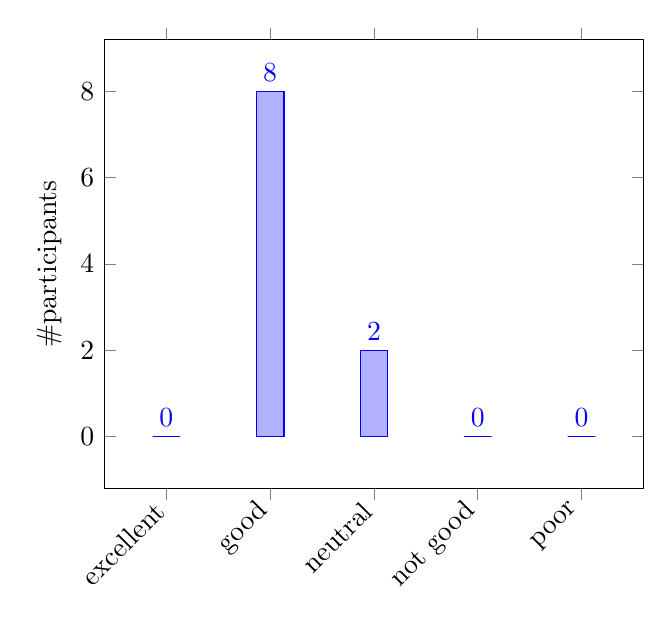
\begin{tikzpicture}
        \begin{axis}[
          ybar,
          enlargelimits=0.15,
          legend style={at={(0.5,-0.2)},
            anchor=north,legend columns=-1},
          ylabel={\#participants},
          symbolic x coords={excellent,good,neutral,%
            not good,poor},
          xtick=data,
          nodes near coords,
          nodes near coords align={vertical},
          x tick label style={rotate=45,anchor=east},
          ]
          \addplot coordinates {(excellent,0) (good,8)
            (neutral,2) (not good,0) (poor,0)};
        \end{axis}
      \end{tikzpicture}}
  \end{floatrow}
\end{figure*}

\begin{figure*}[h]
  \centering
  \begin{floatrow}[3]
    \ffigbox[\FBwidth+1.5cm]
    {\caption{Bar Chart}\label{fig7}}
    {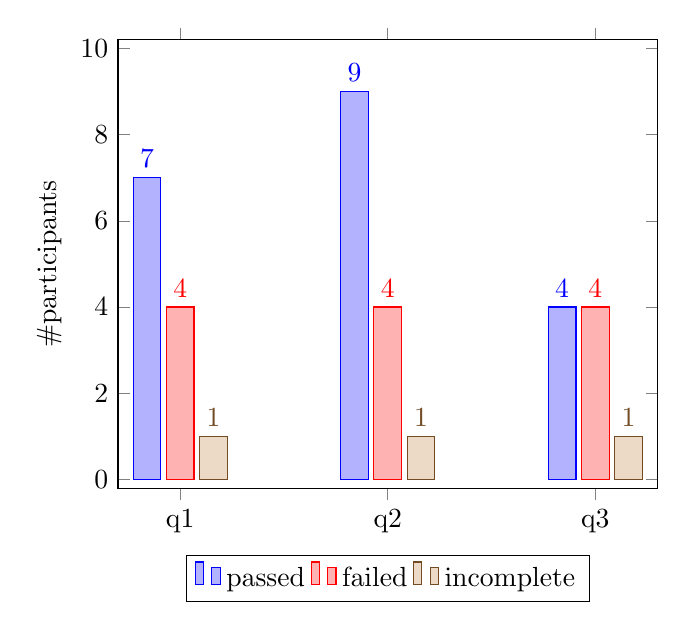
\begin{tikzpicture}
        \begin{axis}[
          ybar,
          enlargelimits=0.15,
          legend style={at={(0.5,-0.15)},
            anchor=north,legend columns=-1},
          ylabel={\#participants},
          symbolic x coords={q1,q2,q3},
          xtick=data,
          nodes near coords,
          nodes near coords align={vertical},
          ]
          \addplot coordinates {(q1,7) (q2,9) (q3,4)};
          \addplot coordinates {(q1,4) (q2,4) (q3,4)};
          \addplot coordinates {(q1,1) (q2,1) (q3,1)};
          \legend{passed,failed,incomplete}
        \end{axis}
      \end{tikzpicture}}
    \ffigbox[\FBwidth+3cm][\FBheight-0.3cm]
    {\caption{Bar Chart Grouped by Time Range}\label{fig8}}
    {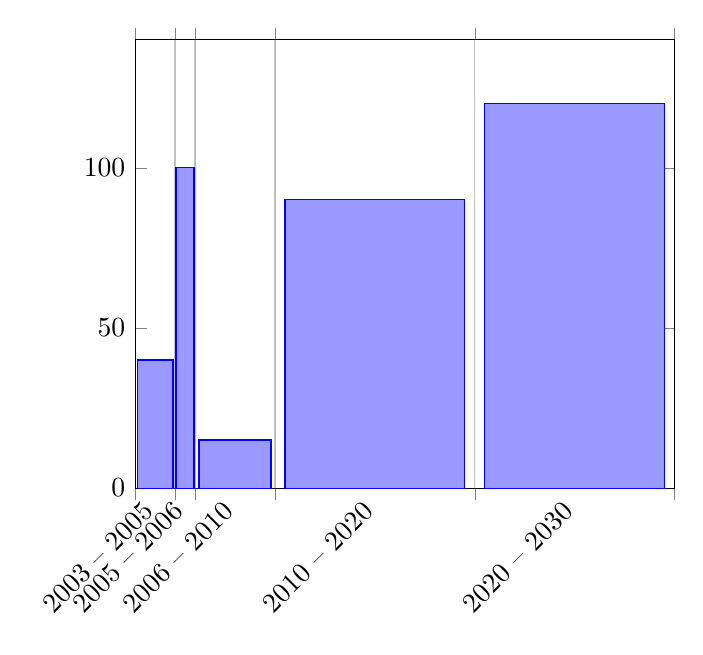
\begin{tikzpicture}
        \begin{axis}[
          ybar interval=0.9,
          x tick label as interval,
          xmin=2003,xmax=2030,
          ymin=0,ymax=140,
          xticklabel={
            $\pgfmathprintnumber{\tick}$
            -- $\pgfmathprintnumber{\nexttick}$},
          xtick=data,
          x tick label style={
            rotate=45,anchor=east,
            /pgf/number format/1000 sep=}]
          \addplot[draw=blue,fill=blue!40!white]
          coordinates
          {(2003,40) (2005,100) (2006,15)
            (2010,90) (2020,120) (2030,3)};
        \end{axis}
      \end{tikzpicture}}
  \end{floatrow}
\end{figure*}

\begin{figure*}[h]
  \centering
  \begin{floatrow}[3]
    \ffigbox[\FBwidth+3cm][\FBheight+1cm]
    {\caption{Scatter Plot}\label{fig9}}
    {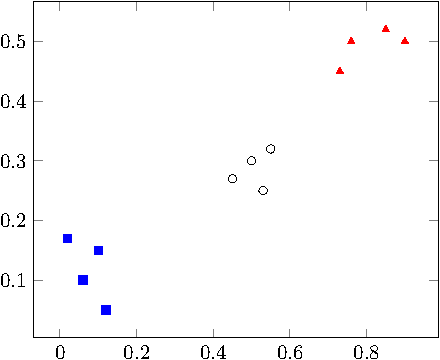
\includegraphics[page=1]{/Users/will/projects/dave/resources/plots/scatter_plot.pdf}}
    \ffigbox[\FBwidth+3cm]
    {\caption{Polar Chart}\label{fig10}}
    {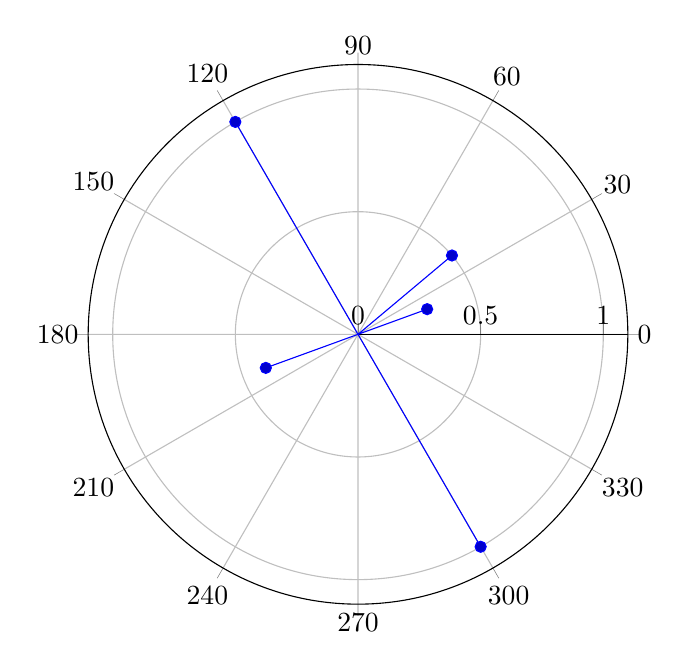
\begin{tikzpicture}
        \begin{polaraxis}
          \addplot+[polar comb]
          coordinates {(300,1) (20,0.3) (40,0.5)
            (120,1) (200,0.4)};
        \end{polaraxis}
      \end{tikzpicture}}
  \end{floatrow}
\end{figure*}

\begin{figure*}[h]
  \centering
  \begin{floatrow}[3]
    \ffigbox[\FBwidth+4cm][\FBheight+1cm]
    {\caption{Gantt Chart}\label{fig11}}
    {\begin{tikzpicture}
        \begin{axis}[xtick=\empty, ytick=\empty]
          \addplot+
          [jump mark left]
          coordinates
          {(0,12) (1,9) (2,8) (3,5) (4,3) (5,1)};
        \end{axis}
      \end{tikzpicture}}
    \ffigbox[\FBwidth+3cm]
    {\caption{Heat Map}\label{fig12}}
    {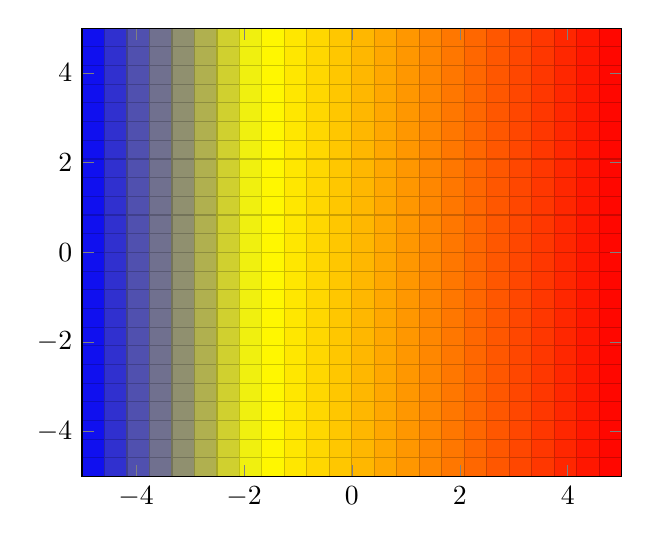
\begin{tikzpicture}
	\begin{axis}[view={0}{90}]
          \addplot3[surf] {x};
	\end{axis}
      \end{tikzpicture}}
  \end{floatrow}
\end{figure*}

\begin{figure}[h]
  \centering
  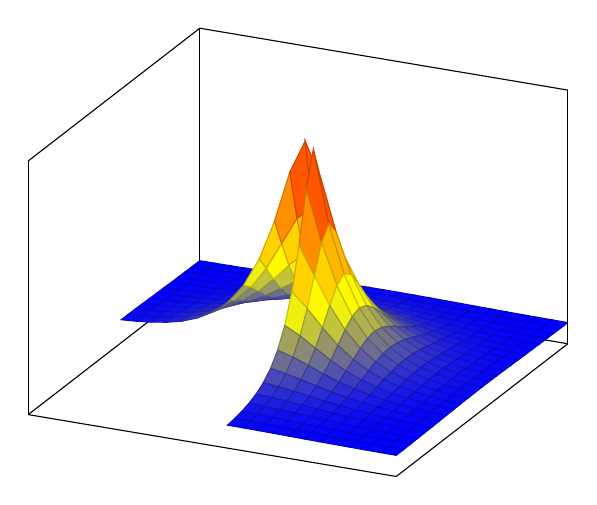
\begin{tikzpicture}
    \begin{axis}[
      xtick=\empty, ytick=\empty, ztick=\empty,
      unbounded coords=jump,
      % A technical filter to cut out
      % the x<0 and y<0 edge.
      filter point/.code={%
        \pgfmathparse
        {\pgfkeysvalueof{/data point/x}<0}%
        \ifpgfmathfloatcomparison
        \pgfmathparse
        {\pgfkeysvalueof{/data point/y}<0}%
        \ifpgfmathfloatcomparison
        \pgfkeyssetvalue{/data point/x}{nan}%
        \fi
        \fi
      },
      ]
      \addplot3[surf] {exp(-sqrt(x^2 + y^2))};
    \end{axis}
  \end{tikzpicture}
  \caption{3D Plot}
\end{figure}

\begin{figure}[h]
  \centering
  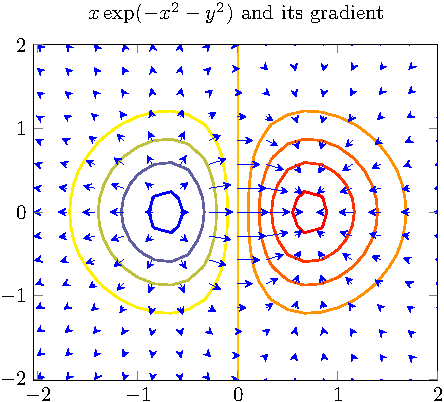
\includegraphics[page=1]{/Users/will/projects/dave/resources/plots/gradient.pdf}
  \caption{Gradient plot}
\end{figure}

\end{document}
